\documentclass[aspectratio=169,10pt]{beamer}
\usetheme{mekatronik}
\renewcommand{\coursetitle}{Mechatronics and Robotics Engineering (50 h)}
\setweek{1}
\setday{4}{Control (cont.) + Servo Systems I}
\title[Control (cont.) \& Servo Systems I]{Control (cont.) and Servo Systems I}
\subtitle{2.7 Filters \& compensation $\cdot$ 2.8 Digital control $\cdot$ 2.9 Control of robot manipulators $\cdot$ 3.1 Servo architecture \& modes $\cdot$ 3.2 Power electronics for drives}
\author{Mechatronics and Robotics Engineering Programme}
\institute{Week 1 \textperiodcentered{} Day 4}
\date{2 weeks \textperiodcentered{} 10 days \textperiodcentered{} 50 hours}

% ------------------------------------------------------------------ local styles
\tikzset{
  blk/.style={draw=mkBlue,fill=mkPale,rounded corners=1pt,minimum height=6.5mm,minimum width=9mm,
              font=\scriptsize,align=center,inner sep=2pt},
  blkO/.style={blk,draw=mkOrange,fill=mkCream},
  blkG/.style={blk,draw=mkGray,fill=mkLight,dashed},
  sumn/.style={draw=mkBlue,circle,inner sep=0pt,minimum size=3.6mm,fill=white},
  sig/.style={-{Latex[length=1.5mm]},mkNavy,line width=.55pt},
  lbl/.style={font=\tiny,text=mkGray},
}
\newcommand{\src}[1]{\par\vspace{1mm}{\color{mkGray}\fontsize{6}{7}\selectfont #1\par}}
\newcommand{\sumsym}{\scalebox{.7}{$\Sigma$}}
\newcommand{\gofurther}[1]{\par\vspace{1mm}{\scriptsize\color{mkGray}\textbf{\color{mkMid}Going further:} #1\par}}
\pgfplotsset{every axis/.append style={label style={font=\scriptsize}}}

\begin{document}

% ==================================================================== TITLE
\begin{frame}[plain]\titlepage\end{frame}

% ==================================================================== AGENDA
\begin{frame}{Agenda and learning outcomes}
\begin{columns}[T]
\begin{column}{.50\textwidth}
\small
\begin{tabular}{@{}l l r@{}}
\toprule
\textbf{Code} & \textbf{Session} & \textbf{Time}\\
\midrule
2.7 & Filters and compensation & 60 min\\
2.8 & Digital control & 60 min\\
2.9 & Control of robot manipulators & 60 min\\
3.1 & Servo architecture and control modes & 60 min\\
3.2 & Power electronics for drives & 60 min\\
\midrule
 & \textbf{Net teaching time} & \textbf{5 h}\\
\bottomrule
\end{tabular}

\vspace{2mm}
{\scriptsize\color{mkGray}Short breaks ($\approx$10 min) after each 1-h block are extra.}
\end{column}
\begin{column}{.48\textwidth}
\begin{keybox}[By the end of today you can \dots]
\small
\checkitem\ \textbf{calculate} the phase a filter or a sampling delay costs a loop\\[.5mm]
\checkitem\ \textbf{choose} a notch or lead compensator for a given problem\\[.5mm]
\checkitem\ \textbf{explain} gravity compensation and computed torque for a robot arm\\[.5mm]
\checkitem\ \textbf{sketch} a servo drive with its torque, velocity and position loops\\[.5mm]
\checkitem\ \textbf{calculate} DC-bus voltage, PWM average voltage and braking energy
\end{keybox}
\end{column}
\end{columns}
\end{frame}

% ==================================================================== RECAP
\begin{frame}{What we learned so far (W1D3 in one slide)}
\begin{columns}[T]
\begin{column}{.48\textwidth}
\centering
\begin{tikzpicture}
  \node[sumn] (S) {\sumsym};
  \node[blk,right=6mm of S] (C) {$C(s)$\\[-.5mm]\tiny PID};
  \node[blk,right=6mm of C] (G) {$G(s)$\\[-.5mm]\tiny joint};
  \draw[sig] ($(S.west)+(-6mm,0)$) node[left,font=\scriptsize]{$r$} -- (S);
  \draw[sig] (S) -- node[above,font=\tiny]{$e$} (C);
  \draw[sig] (C) -- node[above,font=\tiny]{$u$} (G);
  \draw[sig] (G.east) -- ++(7mm,0) node[right,font=\scriptsize]{$y$};
  \draw[sig] ($(G.east)+(3.5mm,0)$) -- ++(0,-8mm) -| node[pos=.95,left,font=\tiny]{$-$} (S);
\end{tikzpicture}

\vspace{1mm}
\small
\begin{itemize}\setlength\itemsep{.4mm}
\item \term{feedback}: measure $y$, compare with $r$, correct
\item \term{PID}: P reacts to the error now, I to its history, D to its trend
\item \term{anti-windup}: stop the integrator when the output saturates
\end{itemize}
\end{column}
\begin{column}{.50\textwidth}
\small
\begin{itemize}\setlength\itemsep{.4mm}
\item \term{Bode plot}: gain and phase of the loop $L(j\omega)=C\,G$
\item \term{crossover} $\omega_c$: where $|L|=1$ (0\,dB) $\approx$ bandwidth
\item \term{phase margin} PM $=180^\circ+\angle L(j\omega_c)$; aim for 45--60$^\circ$
\end{itemize}
\begin{keybox}[Today's thread]
Filters, sampling delay and resonances \hl{cost phase}; lead compensators and fast sampling \hl{buy it back}. Then we open the box: the servo drive that runs these loops.
\end{keybox}
\end{column}
\end{columns}
\end{frame}

% ####################################################################
\section{2.7 Filters and Compensation}
% ####################################################################

\begin{frame}{Refresher: what does a filter do?}
\begin{columns}[T]
\begin{column}{.48\textwidth}
\begin{defbox}[Refresher: a filter is a music equaliser]
\small
A \term{filter} passes some frequencies and weakens others.
\begin{itemize}\setlength\itemsep{0mm}
\item \term{low-pass} (LPF): treble down, bass kept
\item \term{high-pass}: bass down (removes offsets)
\item \term{notch}: removes one tone (a hum)
\end{itemize}
\end{defbox}
\small
\vspace{-1mm}
\begin{eqbox}
\[ |F(f)|=\frac{1}{\sqrt{1+(f/f_f)^2}},\qquad f_f=\frac{1}{2\pi RC}\ \text{[Hz]} \]
\end{eqbox}
RC low-pass: $R=\SI{1}{k\ohm}$, $C=\SI{1}{\micro F}$ $\Rightarrow$ $f_f=\SI{159}{Hz}$; at \SI{1.59}{kHz} only 10\,\% passes.
\end{column}
\begin{column}{.50\textwidth}
\centering
\begin{tikzpicture}
\begin{axis}[mkplot,xmode=log,width=7.2cm,height=4.3cm,xmin=0.01,xmax=100,ymin=-45,ymax=5,
  xlabel={frequency $f/f_f$},ylabel={gain [dB]},legend style={at={(0.03,0.03)},anchor=south west,font=\tiny}]
\addplot[mkBlue,thick,domain=-2:2,samples=120] ({10^x},{-10*log10(1+10^(2*x))});\addlegendentry{low-pass}
\addplot[mkOrange,thick,domain=-2:2,samples=120] ({10^x},{20*x-10*log10(1+10^(2*x))});\addlegendentry{high-pass}
\addplot[mkMid,thick,densely dashed,domain=-2:2,samples=200] ({10^x},{10*log10(((1-10^(2*x))^2+(0.04*10^x)^2)/((1-10^(2*x))^2+(10^x)^2))});\addlegendentry{notch}
\end{axis}
\end{tikzpicture}

\begin{keybox}[Take-away]
Every filter that weakens a signal also \hl{delays} it a little. Inside a control loop that delay is a cost.
\end{keybox}
\end{column}
\end{columns}
\end{frame}

% --------------------------------------------------------------------
\begin{frame}{Why filters in a robot joint loop --- and where they sit}
\begin{columns}[T]
\begin{column}{.58\textwidth}
\centering
\begin{tikzpicture}[node distance=5mm]
  \node[blkO] (Fr) {$F_r(s)$\\[-.5mm]\tiny reference};
  \node[sumn,right=4mm of Fr] (S) {\sumsym};
  \node[blk,right=5mm of S] (C) {$C(s)$};
  \node[blkO,right=4mm of C] (Fu) {$F_u(s)$\\[-.5mm]\tiny torque cmd};
  \node[blk,right=4mm of Fu] (G) {$G(s)$\\[-.5mm]\tiny joint};
  \node[blkO,below=7mm of C] (Fy) {$F_y(s)$\\[-.5mm]\tiny feedback};
  \node[blk,right=4mm of Fy,minimum width=8mm] (Sen) {encoder};
  \draw[sig] ($(Fr.west)+(-5mm,0)$) node[left,font=\scriptsize]{$r$} -- (Fr);
  \draw[sig] (Fr) -- (S);
  \draw[sig] (S) -- (C);
  \draw[sig] (C) -- (Fu);
  \draw[sig] (Fu) -- (G);
  \draw[sig] (G.east) -- ++(5mm,0) node[right,font=\scriptsize]{$y$};
  \draw[sig] ($(G.east)+(2.5mm,0)$) |- (Sen);
  \draw[sig] (Sen) -- (Fy);
  \draw[sig] (Fy) -| node[pos=.95,left,font=\tiny]{$-$} (S);
  \node[font=\tiny,text=mkRed,above=5mm of C.north,anchor=south] {inside the loop: costs phase at $\omega_c$};
  \draw[mkRed,densely dotted] ($(S.north)+(-1mm,4mm)$) rectangle ($(G.south east)+(1mm,-1.6cm)$);
  \node[font=\tiny,text=mkGreen,below=1.5mm of Fr] {outside: free};
\end{tikzpicture}
\end{column}
\begin{column}{.40\textwidth}
\small
\textbf{What we filter against}
\begin{itemize}\setlength\itemsep{.3mm}
\item encoder quantisation noise (``steps'')
\item resonances of gearboxes, belts, long links
\item jerky set-points from the robot program
\item offsets of analogue sensors
\end{itemize}
\end{column}
\end{columns}
\vspace{2mm}
\begin{keybox}[Rule]
A filter \hl{inside} the loop ($F_u$, $F_y$) becomes part of $L(s)$ and eats phase margin. A filter on the reference ($F_r$) only shapes the motion --- no stability cost.
\end{keybox}
\end{frame}

% --------------------------------------------------------------------
\begin{frame}{Low-pass filter: cut-off, order and phase}
\begin{columns}[T]
\begin{column}{.43\textwidth}
\small
\begin{eqbox}
\[ F_1(s)=\frac{\omega_f}{s+\omega_f} \]
\end{eqbox}
\begin{itemize}\setlength\itemsep{.4mm}
\item \term{cut-off} $\omega_f$ [rad/s]: the $-3$\,dB point
\item \term{order} $n$: roll-off $-20n$\,dB per decade
\item phase: $-45^\circ$ per order at $\omega_f$
\item 2nd order with low damping \hl{peaks} near $\omega_f$
\end{itemize}
\textbf{Take-away:} higher order = cleaner signal, but much more phase lag.
\end{column}
\begin{column}{.55\textwidth}
\centering
\begin{tikzpicture}
\begin{groupplot}[group style={group size=1 by 2,vertical sep=2mm,xticklabels at=edge bottom},
  mkplot,xmode=log,width=7.4cm,height=3.35cm,xmin=0.01,xmax=100]
\nextgroupplot[ylabel={$|F|$ [dB]},ymin=-90,ymax=8,ytick={-80,-60,-40,-20,0},
  legend style={at={(0.02,0.05)},anchor=south west,font=\tiny}]
\addplot table[x=w,y=m1]{data/lpf_bode.dat};\addlegendentry{1st order}
\addplot table[x=w,y=m2]{data/lpf_bode.dat};\addlegendentry{2nd order}
\addplot table[x=w,y=m4]{data/lpf_bode.dat};\addlegendentry{4th order}
\nextgroupplot[ylabel={$\angle F$ [$^\circ$]},xlabel={$\omega/\omega_f$},ymin=-370,ymax=10,ytick={-360,-270,-180,-90,0}]
\addplot table[x=w,y=p1]{data/lpf_bode.dat};
\addplot table[x=w,y=p2]{data/lpf_bode.dat};
\addplot table[x=w,y=p4]{data/lpf_bode.dat};
\draw[mkGray,densely dashed] (axis cs:1,-370) -- (axis cs:1,10);
\end{groupplot}
\end{tikzpicture}
\end{column}
\end{columns}
\end{frame}

% --------------------------------------------------------------------
\begin{frame}{The price of filtering: phase lost at crossover}
\begin{columns}[T]
\begin{column}{.47\textwidth}
\centering
\begin{tikzpicture}
\begin{axis}[mkplot,xmode=log,width=6.6cm,height=4.6cm,xmin=1,xmax=30,ymin=0,ymax=90,
   xlabel={ratio $\omega_f/\omega_c$},ylabel={phase lost at $\omega_c$ [$^\circ$]},
   xtick={1,2,5,10,20,30},xticklabels={1,2,5,10,20,30},legend style={at={(0.97,0.97)},anchor=north east,font=\tiny}]
\addplot table[x=r,y=p1]{data/phase_loss.dat};\addlegendentry{1st order}
\addplot table[x=r,y=p2]{data/phase_loss.dat};\addlegendentry{2nd order}
\addplot table[x=r,y=p4]{data/phase_loss.dat};\addlegendentry{4th order}
\draw[mkRed,densely dashed] (axis cs:1,10) -- (axis cs:30,10) node[pos=.02,above,font=\tiny,anchor=south west]{10$^\circ$ budget};
\end{axis}
\end{tikzpicture}
\end{column}
\begin{column}{.51\textwidth}
\small
\begin{eqbox}
\[ \Delta\varphi=\arctan\frac{\omega_c}{\omega_f}\quad\text{(1st-order LPF)} \]
\end{eqbox}
\textbf{Worked example.} Joint velocity loop, $f_c=150$\,Hz; we allow $10^\circ$ of phase loss.
\begin{enumerate}\setlength\itemsep{.3mm}
\item need $f_c/f_f\le\tan10^\circ=0.176$
\item $f_f\ge 150\,\text{Hz}/0.176=\SI{850}{Hz}$
\item check: $\arctan(150/850)=10.0^\circ$ \checkmark
\end{enumerate}
\end{column}
\end{columns}
\vspace{1mm}
\begin{keybox}[Trade-off]
Lower $\omega_f$ = quieter motor but less phase margin. Rule of thumb: $\omega_f\approx(5\ldots10)\,\omega_c$.
\end{keybox}
\end{frame}

% --------------------------------------------------------------------
\begin{frame}{Notch filter: cutting out one frequency}
\begin{columns}[T]
\begin{column}{.45\textwidth}
\small
\textbf{Picture:} a playground swing has one natural frequency --- so does a robot joint with a springy gearbox. A \term{notch} stops the controller ``pushing'' at exactly that frequency.
\begin{eqbox}
\[ N(s)=\frac{s^2+2\zeta_z\omega_n s+\omega_n^2}{s^2+2\zeta_p\omega_n s+\omega_n^2} \]
\end{eqbox}
\begin{itemize}\setlength\itemsep{.3mm}
\item \term{centre} $\omega_n$: set to the resonance
\item \term{depth}: ratio $\zeta_z/\zeta_p$ (0.1 $\rightarrow$ $-20$\,dB)
\item \term{width}: set by $\zeta_p$; wide = robust, more lag
\end{itemize}
\end{column}
\begin{column}{.53\textwidth}
\centering
\begin{tikzpicture}
\begin{groupplot}[group style={group size=1 by 2,vertical sep=2mm,xticklabels at=edge bottom},
  mkplot,xmode=log,width=7.1cm,height=3.35cm,xmin=0.1,xmax=10]
\nextgroupplot[ylabel={$|N|$ [dB]},ymin=-45,ymax=3,legend style={at={(0.02,0.04)},anchor=south west,font=\tiny}]
\addplot table[x=w,y=m1]{data/notch_bode.dat};\addlegendentry{$\zeta_z/\zeta_p=0.01$}
\addplot table[x=w,y=m2]{data/notch_bode.dat};\addlegendentry{$0.1$}
\addplot table[x=w,y=m3]{data/notch_bode.dat};\addlegendentry{$0.3$}
\nextgroupplot[ylabel={$\angle N$ [$^\circ$]},xlabel={$\omega/\omega_n$ \quad ($\zeta_p=0.5$)},ymin=-95,ymax=95,ytick={-90,-45,0,45,90}]
\addplot table[x=w,y=p1]{data/notch_bode.dat};
\addplot table[x=w,y=p2]{data/notch_bode.dat};
\addplot table[x=w,y=p3]{data/notch_bode.dat};
\end{groupplot}
\end{tikzpicture}
\end{column}
\end{columns}
\end{frame}

% --------------------------------------------------------------------
\begin{frame}{Notch in practice: taming a 1\,kHz resonance}
\begin{columns}[T]
\begin{column}{.40\textwidth}
\small
\textbf{Axis:} motor -- stiff coupling -- load, resonance at $f_r=\SI{1}{kHz}$. Velocity PI with $f_c=\SI{100}{Hz}$.

\vspace{1mm}
\begin{tabular}{@{}lcc@{}}
\toprule
 & no notch & notch\\
\midrule
0\,dB crossings & 3 & 1\\
PM at 100\,Hz & $65^\circ$ & $61^\circ$\\
closed loop & \textcolor{mkRed}{unstable} & \textcolor{mkGreen}{stable}\\
\bottomrule
\end{tabular}

\vspace{1mm}
The resonance lifts $|L|$ above 0\,dB near 1\,kHz with no phase left. A $-25$\,dB notch removes the peak and costs only $\approx4^\circ$ at 100\,Hz.
\end{column}
\begin{column}{.58\textwidth}
\centering
\begin{tikzpicture}
\begin{groupplot}[group style={group size=1 by 2,vertical sep=2mm,xticklabels at=edge bottom},
  mkplot,xmode=log,width=8.3cm,height=3.45cm,xmin=10,xmax=3000]
\nextgroupplot[ylabel={$|L|$ [dB]},ymin=-50,ymax=40,legend style={at={(0.98,0.97)},anchor=north east,font=\tiny}]
\addplot table[x=f,y=m0]{data/notch_app.dat};\addlegendentry{without notch}
\addplot table[x=f,y=m1]{data/notch_app.dat};\addlegendentry{with notch}
\draw[mkRed,thin] (axis cs:10,0) -- (axis cs:3000,0);
\nextgroupplot[ylabel={$\angle L$ [$^\circ$]},xlabel={$f$ [Hz]},ymin=-400,ymax=0,ytick={-360,-270,-180,-90,0}]
\addplot table[x=f,y=p0]{data/notch_app.dat};
\addplot table[x=f,y=p1]{data/notch_app.dat};
\draw[mkRed,thin] (axis cs:10,-180) -- (axis cs:3000,-180);
\end{groupplot}
\end{tikzpicture}
\end{column}
\end{columns}
\src{Model and numbers computed for this course; cf.\ [Ellis, 2012, ch.~16]. Joint resonances return in W2D1 (session 3.7).}
\end{frame}

% --------------------------------------------------------------------
\begin{frame}{Phase-lead compensator: buying phase back}
\begin{columns}[T]
\begin{column}{.46\textwidth}
\small
\begin{eqbox}
\[ C_{\text{lead}}(s)=K\,\frac{1+\alpha T s}{1+T s},\qquad \alpha>1 \]
\end{eqbox}
\begin{itemize}\setlength\itemsep{.4mm}
\item a zero before a pole: phase goes \hl{up} between them
\item maximum lead at $\omega_m=1/(T\sqrt\alpha)$ --- put it at $\omega_c$
\item $\alpha=3\rightarrow30^\circ$, $\alpha=7.5\rightarrow50^\circ$, $\alpha=20\rightarrow65^\circ$
\item price: high-frequency gain $\times\alpha$ $\Rightarrow$ more noise
\end{itemize}
\textbf{Picture:} steering a bicycle by looking ahead --- the lead reacts to where the error is \emph{going}.
\end{column}
\begin{column}{.52\textwidth}
\centering
\begin{tikzpicture}
\begin{groupplot}[group style={group size=1 by 2,vertical sep=2mm,xticklabels at=edge bottom},
  mkplot,xmode=log,width=7.2cm,height=3.35cm,xmin=0.01,xmax=100]
\nextgroupplot[ylabel={$|C/K|$ [dB]},ymin=-2,ymax=28,legend style={at={(0.02,0.97)},anchor=north west,font=\tiny}]
\addplot table[x=w,y=m3]{data/lead_family.dat};\addlegendentry{$\alpha=3$}
\addplot table[x=w,y=m7]{data/lead_family.dat};\addlegendentry{$\alpha=7.55$}
\addplot table[x=w,y=m20]{data/lead_family.dat};\addlegendentry{$\alpha=20$}
\nextgroupplot[ylabel={$\angle C$ [$^\circ$]},xlabel={$\omega/\omega_m$},ymin=0,ymax=70,ytick={0,30,50,65}]
\addplot table[x=w,y=p3]{data/lead_family.dat};
\addplot table[x=w,y=p7]{data/lead_family.dat};
\addplot table[x=w,y=p20]{data/lead_family.dat};
\draw[mkGray,densely dashed] (axis cs:1,0) -- (axis cs:1,70);
\end{groupplot}
\end{tikzpicture}
\end{column}
\end{columns}
\src{[Ogata, 2010, ch.~7]; [Franklin, Powell \& Emami-Naeini, 2019, ch.~6].}
\end{frame}

% --------------------------------------------------------------------
\begin{frame}{Lead design --- worked example: position loop on a pure inertia}
\begin{columns}[T]
\begin{column}{.48\textwidth}
\small
Plant $G=1/(Js^2)$, $J=\SI{2e-4}{kg\,m^2}$: phase is $-180^\circ$ everywhere, so PM $=0$ with a plain gain.
\textbf{Goal:} $f_c=\SI{50}{Hz}$ ($\omega_c=\SI{314}{rad/s}$), PM $=50^\circ$.
\begin{enumerate}\setlength\itemsep{.4mm}
\item need $50^\circ$ of lead $\Rightarrow\alpha=7.55$ (graph)
\item centre it: $T=1/(\omega_c\sqrt\alpha)=\SI{1.16}{ms}$
\item gain for $|L|=1$ at $\omega_c$: $K=J\omega_c^2/\sqrt\alpha=\SI{7.2}{N\,m/rad}$
\item check (computed): $f_c=\SI{49.5}{Hz}$, PM $=50^\circ$ \checkmark
\end{enumerate}
Step overshoot 28\,\% (from the lead zero); a reference filter $F_r$ can remove it.
\end{column}
\begin{column}{.50\textwidth}
\centering
\begin{tikzpicture}
\begin{groupplot}[group style={group size=1 by 2,vertical sep=10mm},mkplot,width=7.0cm,height=3.25cm]
\nextgroupplot[xmode=log,xmin=1,xmax=10000,ymin=-200,ymax=-120,ylabel={$\angle L$ [$^\circ$]},xlabel={$f$ [Hz]},
   ytick={-180,-160,-140,-130}]
\addplot[mkBlue,thick] table[x=f,y=pL]{data/lead_bode.dat};
\draw[mkRed,thin] (axis cs:1,-180) -- (axis cs:10000,-180);
\draw[mkOrange,thick,{Latex[length=1.2mm]}-{Latex[length=1.2mm]}] (axis cs:49.5,-180) -- (axis cs:49.5,-130) node[midway,right,font=\tiny]{PM $=50^\circ$};
\nextgroupplot[xmin=0,xmax=30,ymin=0,ymax=1.4,xlabel={$t$ [ms]},ylabel={$\theta/\theta_{\text{ref}}$}]
\addplot[mkOrange,thick] table[x=t,y=y]{data/lead_step.dat};
\draw[mkGray,densely dashed] (axis cs:0,1) -- (axis cs:30,1);
\end{groupplot}
\end{tikzpicture}
\end{column}
\end{columns}
\end{frame}

% --------------------------------------------------------------------
\begin{frame}{Phase-lag compensator and lead--lag}
\begin{columns}[T]
\begin{column}{.47\textwidth}
\small
\begin{eqbox}
\[ C_{\text{lag}}(s)=\beta\,\frac{1+T s}{1+\beta T s},\qquad \beta>1 \]
\end{eqbox}
\begin{itemize}\setlength\itemsep{.4mm}
\item boosts gain at \hl{low} frequency by $\beta$ $\Rightarrow$ smaller steady error, stiffer against load
\item leaves high frequencies (and noise) alone
\item zero a decade below $\omega_c$: costs only $\approx5^\circ$
\item \term{lead--lag}: lead buys PM, lag buys stiffness
\end{itemize}
\begin{notebox}
\small PID is a lead--lag in disguise: PI $\approx$ lag, filtered D $\approx$ lead.
\end{notebox}
\end{column}
\begin{column}{.51\textwidth}
\centering
\begin{tikzpicture}
\begin{groupplot}[group style={group size=1 by 2,vertical sep=2mm,xticklabels at=edge bottom},
  mkplot,xmode=log,width=7.1cm,height=3.35cm,xmin=0.01,xmax=100]
\nextgroupplot[ylabel={$|C_{\text{lag}}|$ [dB]},ymin=-3,ymax=23]
\addplot[mkBlue,thick] table[x=w,y=m]{data/lag_bode.dat};
\node[font=\tiny,anchor=west] at (axis cs:0.012,17) {$+20\log\beta$};
\draw[mkGray,densely dashed] (axis cs:10,-3) -- (axis cs:10,23) node[pos=.6,right,font=\tiny]{$\omega_c$};
\nextgroupplot[ylabel={$\angle C_{\text{lag}}$ [$^\circ$]},xlabel={$\omega T$ \quad($\beta=10$)},ymin=-60,ymax=5]
\addplot[mkBlue,thick] table[x=w,y=p]{data/lag_bode.dat};
\draw[mkGray,densely dashed] (axis cs:10,-60) -- (axis cs:10,5);
\end{groupplot}
\end{tikzpicture}
\end{column}
\end{columns}
\gofurther{a \term{high-pass} filter $s/(s+\omega_h)$ removes offsets (e.g.\ accelerometer drift) but must never sit in the main position feedback path.}
\end{frame}

% --------------------------------------------------------------------
\begin{frame}{Session 2.7 --- Check your understanding}
\begin{keybox}[Check your understanding]
\begin{enumerate}\setlength\itemsep{2mm}
\item A colleague adds a 4th-order low-pass at $2\,f_c$ to the joint velocity feedback ``to clean it up''. What happens to the phase margin?
\item Why does a reference filter $F_r$ not change stability, while a feedback filter $F_y$ does?
\item The robot joint whistles at 800\,Hz when you raise the gain. Which filter do you reach for, and where do you set its centre?
\end{enumerate}
\end{keybox}
\vspace{2mm}
{\small\color{mkGray}Discuss in pairs for 2 minutes, then we compare answers.}
\end{frame}

% --------------------------------------------------------------------
\begin{frame}{Session 2.7 --- Summary and key terms}
\begin{columns}[T]
\begin{column}{.52\textwidth}
\begin{keybox}[Key take-aways]
\begin{itemize}\setlength\itemsep{.3mm}
\item In-loop filters are part of $L(s)$: budget their phase ($\omega_f\approx5$--$10\,\omega_c$).
\item A notch removes one resonance for a few degrees of PM.
\item Lead adds phase at $\omega_c$; lag adds low-frequency stiffness.
\item Reference filters are ``free'': they shape motion, not stability.
\end{itemize}
\end{keybox}
\end{column}
\begin{column}{.46\textwidth}
\begin{defbox}[Key terms]
\small
\term{cut-off} $-3$\,dB frequency $\cdot$ \term{order} steepness of roll-off $\cdot$ \term{low/high-pass} keeps slow/fast parts $\cdot$ \term{notch} removes one frequency $\cdot$ \term{resonance} frequency where a structure swings strongly $\cdot$ \term{lead/lag} compensator adding phase / low-frequency gain
\end{defbox}
\end{column}
\end{columns}
\end{frame}

% ####################################################################
\section{2.8 Digital Control}
% ####################################################################

\begin{frame}{Refresher: sampling a signal}
\begin{columns}[T]
\begin{column}{.46\textwidth}
\begin{defbox}[Refresher: sampling is taking snapshots]
\small
A film shows motion as 24 photos per second. A digital controller sees a signal only at the instants $t=kT$:
\[ f_s=\frac1T\quad\text{[Hz]},\qquad y_k=y(kT) \]
Between samples the output is \term{held} constant: the \term{zero-order hold} (ZOH) makes a staircase.
\end{defbox}
\small
\textbf{Example:} $f_s=8$\,kHz $\Rightarrow T=\SI{125}{\micro s}$; a 100\,Hz sine gets 80 samples per period.
\end{column}
\begin{column}{.52\textwidth}
\centering
\begin{tikzpicture}
\begin{axis}[mkplot,width=7.6cm,height=4.6cm,xmin=0,xmax=1,ymin=-1.5,ymax=1.5,xlabel={$t/T_0$ \quad ($T=T_0/12$)},ylabel={signal},
  legend style={at={(0.99,0.99)},anchor=north east,font=\tiny}]
\addplot[mkBlue,thick] table[x=t,y=y]{data/zoh_cont.dat};\addlegendentry{$y(t)$}
\addplot[mkOrange,thick,const plot] table[x=t,y=y]{data/zoh_samp.dat};\addlegendentry{held samples}
\addplot[mkSky,thick,densely dashed] table[x=t,y=yd]{data/zoh_cont.dat};\addlegendentry{$y(t-T/2)$}
\addplot[mkOrange,only marks,mark=*,mark size=1.2pt,forget plot] table[x=t,y=y]{data/zoh_samp.dat};
\end{axis}
\end{tikzpicture}
\begin{keybox}[Take-away]
The staircase follows the signal \hl{half a sample late} on average: holding costs a delay of $T/2$.
\end{keybox}
\end{column}
\end{columns}
\end{frame}

% --------------------------------------------------------------------
\begin{frame}{Anatomy of a digital joint controller}
\centering
\begin{tikzpicture}
  \node[sumn] (S) {\sumsym};
  \node[blk,right=6mm of S,minimum width=16mm] (C) {$C(z)$\\[-.5mm]\tiny CPU / FPGA};
  \node[blkO,right=7mm of C,minimum width=14mm] (H) {ZOH\\[-.5mm]\tiny PWM update};
  \node[blk,right=7mm of H,minimum width=16mm] (G) {$G(s)$\\[-.5mm]\tiny drive + motor + link};
  \node[blkO,below=7mm of H,minimum width=14mm] (A) {sampler\\[-.5mm]\tiny ADC / encoder};
  \draw[sig] ($(S.west)+(-6mm,0)$) node[left,font=\scriptsize]{$r_k$} -- (S);
  \draw[sig] (S) -- node[above,font=\tiny]{$e_k$} (C);
  \draw[sig] (C) -- node[above,font=\tiny]{$u_k$} (H);
  \draw[sig] (H) -- node[above,font=\tiny]{$u(t)$} (G);
  \draw[sig] (G.east) -- ++(8mm,0) node[right,font=\scriptsize]{$y(t)$};
  \draw[sig] ($(G.east)+(4mm,0)$) |- (A);
  \draw[sig] (A) -| node[pos=.3,below,font=\tiny]{$y_k$} node[pos=.95,left,font=\tiny]{$-$} (S);
  \draw[mkMid,densely dashed] ($(C.north west)+(-14mm,4mm)$) rectangle ($(H.south east)+(2mm,-18mm)$);
  \node[font=\tiny,text=mkMid,anchor=north west] at ($(C.north west)+(-14mm,4mm)$) {discrete world, period $T$};
\end{tikzpicture}
\vspace{2mm}
\begin{columns}[T]
\begin{column}{.5\textwidth}
\small
\begin{itemize}\setlength\itemsep{.4mm}
\item the computer sees $y$ only at $t=kT$
\item the output is held until the next update
\item computing takes time: $u_k$ is usually applied \hl{one sample later}
\end{itemize}
\end{column}
\begin{column}{.48\textwidth}
\small
\begin{tabular}{@{}lcc@{}}
\toprule
Loop & typical $f_s$ & typical $f_c$\\
\midrule
current & 8--32\,kHz & 1--3\,kHz\\
velocity & 4--16\,kHz & 100--500\,Hz\\
position & 1--8\,kHz & 20--100\,Hz\\
robot path planner & 0.25--1\,kHz & ---\\
\bottomrule
\end{tabular}
\end{column}
\end{columns}
\end{frame}

% --------------------------------------------------------------------
\begin{frame}{Delay budget and phase loss at crossover}
\begin{columns}[T]
\begin{column}{.48\textwidth}
\small
\textbf{Picture:} a shower with a long pipe --- you turn the tap, the temperature changes later, and you overcorrect.
\begin{eqbox}
\[ \Delta\varphi=360^\circ\cdot f_c\cdot T_d,\qquad T_d\approx1.5\,T \]
\end{eqbox}
($T/2$ from the hold + $T$ for computing.)\\[1mm]
\textbf{Worked example:} $f_s=4$\,kHz, $f_c=200$\,Hz.
\begin{enumerate}\setlength\itemsep{.3mm}
\item $T=1/4000=\SI{250}{\micro s}$
\item $T_d=1.5\times250=\SI{375}{\micro s}$
\item $\Delta\varphi=360\cdot200\cdot0.000375=$ \hl{27$^\circ$}
\item at 8\,kHz: $13.5^\circ$ --- double $f_s$, halve the loss
\end{enumerate}
\end{column}
\begin{column}{.50\textwidth}
\centering
\begin{tikzpicture}
\begin{axis}[mkplot,width=7.2cm,height=5.4cm,xmin=0,xmax=500,ymin=0,ymax=60,xlabel={$f_c$ [Hz]},ylabel={$\Delta\varphi$ [$^\circ$] for $T_d=1.5T$},
   legend style={at={(0.03,0.97)},anchor=north west,font=\tiny}]
\addplot[mkRed,thick,domain=0:500] {360*x*1.5/2000};\addlegendentry{$f_s=2$\,kHz}
\addplot[mkOrange,thick,domain=0:500] {360*x*1.5/4000};\addlegendentry{$f_s=4$\,kHz}
\addplot[mkBlue,thick,domain=0:500] {360*x*1.5/8000};\addlegendentry{$f_s=8$\,kHz}
\addplot[mkSky,thick,domain=0:500] {360*x*1.5/16000};\addlegendentry{$f_s=16$\,kHz}
\addplot[mkOrange,only marks,mark=*,mark size=1.6pt,forget plot] coordinates {(200,27)};
\end{axis}
\end{tikzpicture}
\end{column}
\end{columns}
\end{frame}

% --------------------------------------------------------------------
\begin{frame}{From the $s$-plane to the $z$-plane}
\begin{columns}[T]
\begin{column}{.46\textwidth}
\small
In discrete time a pole is a number $z$ that multiplies the signal every sample: $x_{k+1}=z\,x_k$.
\begin{eqbox}
\[ z=e^{sT}\qquad\text{stable}\iff|z|<1 \]
\end{eqbox}
\begin{itemize}\setlength\itemsep{.3mm}
\item $|z|<1$: each sample smaller $\Rightarrow$ decays
\item left half $s$-plane $\rightarrow$ inside the unit circle
\item near $z=1$: slow; near $z=-1$: rings at $f_s/2$
\end{itemize}
\textbf{Example:} $s=-70\pm j71$, $T=1$\,ms $\Rightarrow z\approx0.93\pm j0.07$: inside the circle, stable.
\end{column}
\begin{column}{.52\textwidth}
\centering
\begin{tikzpicture}
\begin{axis}[mkplot,grid=none,axis lines=middle,width=6.6cm,height=6.0cm,xmin=-1.25,xmax=1.25,ymin=-0.15,ymax=1.2,axis equal image,
   xlabel={Re $z$},ylabel={Im $z$},xtick={-1,-0.5,0.5,1},ytick={0.5,1},
   every axis x label/.style={at={(ticklabel* cs:1)},anchor=north east,font=\scriptsize},
   every axis y label/.style={at={(ticklabel* cs:1)},anchor=north west,font=\scriptsize}]
\addplot[mkSky,thin] table[x=x,y=y]{data/zeta.dat};
\addplot[mkAmber,thin] table[x=x,y=y]{data/wn.dat};
\addplot[mkBlue,thick,domain=0:180,samples=90] ({cos(x)},{sin(x)});
\addplot[mkOrange,only marks,mark=x,mark size=2.5pt,thick] coordinates {(0.930,0.0665)};
\node[font=\tiny,text=mkMid,anchor=south] at (axis cs:0.0,1.02) {unit circle = stability limit};
\node[font=\tiny,text=mkOrange,anchor=south] at (axis cs:0.93,0.1) {example};
\end{axis}
\end{tikzpicture}

{\scriptsize\color{mkGray} thin lines: constant damping (blue-grey) and constant frequency (amber)}
\end{column}
\end{columns}
\end{frame}

% --------------------------------------------------------------------
\begin{frame}[fragile]{Discrete PID: a few lines every sample}
\begin{columns}[T]
\begin{column}{.45\textwidth}
\small
Every $T$ seconds the controller runs:
\begin{itemize}\setlength\itemsep{.4mm}
\item \textbf{I}: add up the error, $I_k=I_{k-1}+K_iT\,e_k$
\item \textbf{D}: difference of the measurement, filtered
\item \textbf{saturation}: output limited (max.\ current)
\item \term{anti-windup}: when saturated, stop the integrator growing
\end{itemize}
\textbf{Picture:} the integral is a bucket that collects error; the derivative is the slope between two snapshots.
\end{column}
\begin{column}{.53\textwidth}
\begin{notebox}
\scriptsize
\begin{semiverbatim}
// executed every T (interrupt synced to PWM)
e  = r - y;
I += Ki*T*e;                    // integrate
D  = a*D - b*(y - y_old);       // filtered D on y
y_old = y;              // a=Tf/(Tf+T), b=Kd/(Tf+T)
u  = Kp*e + I + D;
if (u > UMAX)      \{ I -= u - UMAX; u = UMAX; \}
else if (u < -UMAX)\{ I -= u + UMAX; u = -UMAX;\}
write_pwm(u);       // takes effect next period
\end{semiverbatim}
\end{notebox}
{\scriptsize D acts on $-y$ so a step in $r$ does not cause a ``kick''.}
\end{column}
\end{columns}
\gofurther{discretisation methods (forward/backward Euler, Tustin, ZOH equivalent) and frequency pre-warping [Franklin, Powell \& Workman, 1998, ch.~6].}
\end{frame}

% --------------------------------------------------------------------
\begin{frame}{Aliasing: the wagon-wheel effect}
\begin{columns}[T]
\begin{column}{.5\textwidth}
\centering
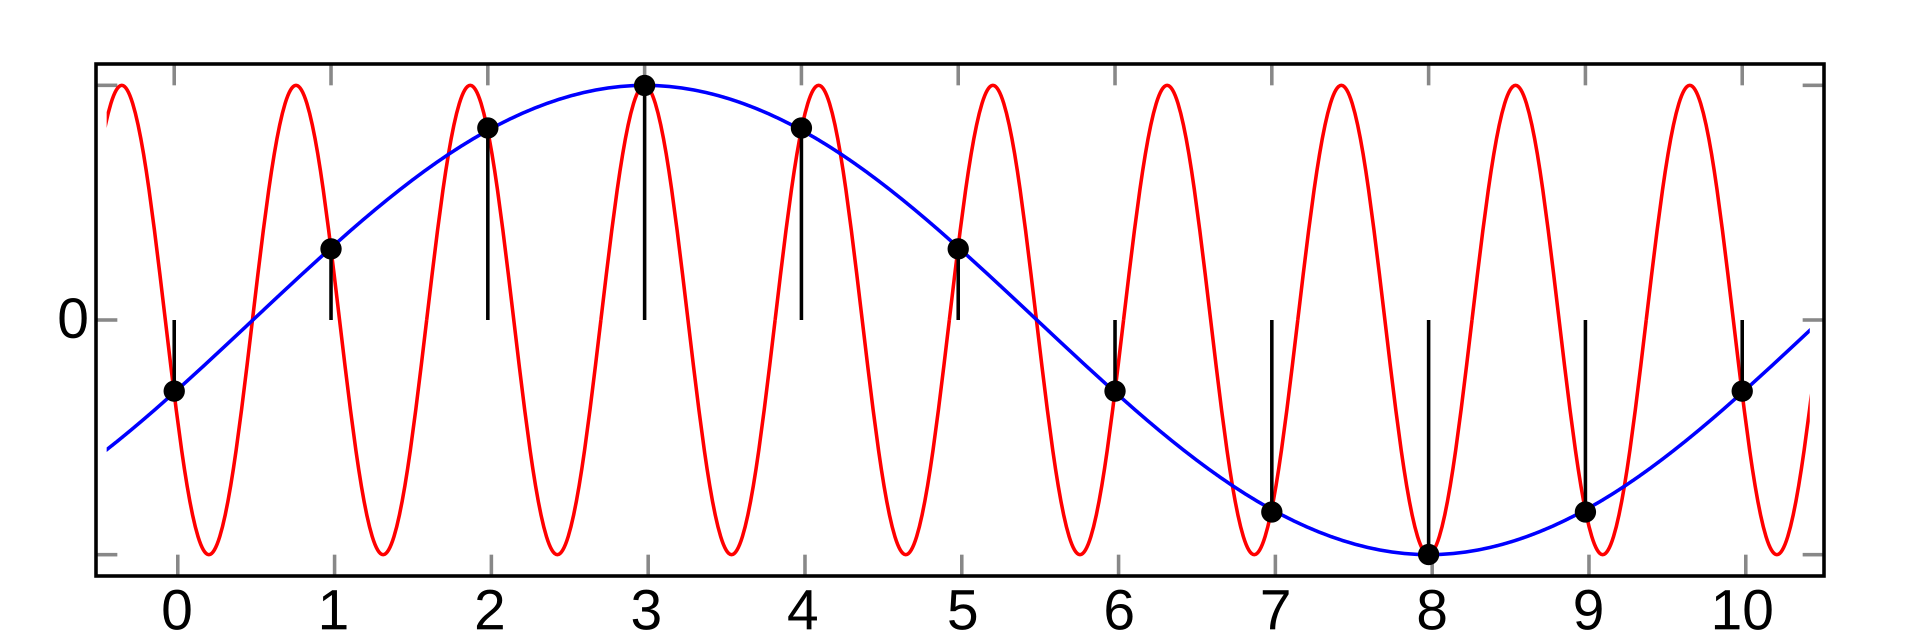
\includegraphics[width=\linewidth]{../../figures/d3_aliasing.png}\\
\credit{Moxfyre, CC BY-SA 3.0, via Wikimedia Commons}\\[1mm]
{\scriptsize red: $f=0.9$, blue: $f=0.1$, sampled at $f_s=1$ --- identical samples}
\end{column}
\begin{column}{.48\textwidth}
\small
\textbf{Picture:} in films a fast wheel seems to turn slowly or backwards --- the camera samples too slowly.
\begin{eqbox}
\[ f_{\text{alias}}=\left|f-k\,f_s\right|,\ \ k=\mathrm{round}(f/f_s) \]
\end{eqbox}
\begin{itemize}\setlength\itemsep{.4mm}
\item anything above $f_s/2$ folds back below it
\item 4.6\,kHz vibration sampled at 4\,kHz looks like \hl{600\,Hz}
\item cure: filter \emph{before} sampling (anti-alias filter)
\end{itemize}
{\scriptsize\color{mkGray}More in W2D5 (session 6.5).}
\end{column}
\end{columns}
\end{frame}

% --------------------------------------------------------------------
\begin{frame}{Choosing the sample rate}
\begin{columns}[T]
\begin{column}{.52\textwidth}
\centering
\begin{tikzpicture}
\begin{axis}[mkplot,width=7.5cm,height=5.4cm,xmin=0,xmax=30,ymin=0,ymax=2.0,xlabel={$t$ [ms]},ylabel={$\omega/\omega_{\text{ref}}$},
   legend style={at={(0.97,0.97)},anchor=north east,font=\tiny}]
\addplot[mkBlue,thick] table[x=t,y=w]{data/fs_20000.dat};\addlegendentry{$f_s=20$\,kHz (14\,\% overshoot)}
\addplot[mkOrange,thick] table[x=t,y=w]{data/fs_4000.dat};\addlegendentry{$f_s=4$\,kHz (16\,\%)}
\addplot[mkRed,thick] table[x=t,y=w]{data/fs_1000.dat};\addlegendentry{$f_s=1$\,kHz (95\,\%)}
\draw[mkGray,densely dashed] (axis cs:0,1) -- (axis cs:30,1);
\end{axis}
\end{tikzpicture}
\end{column}
\begin{column}{.46\textwidth}
\small
Same velocity PI ($f_c=100$\,Hz), only $f_s$ changes.\\[1mm]
At 1\,kHz: $T_d=1.5$\,ms $\Rightarrow\Delta\varphi=360\cdot100\cdot0.0015=54^\circ$ $\Rightarrow$ almost unstable.
\begin{keybox}[Rules of thumb]
\begin{itemize}\setlength\itemsep{.3mm}
\item $f_s\ge 20$--$40\times$ the loop bandwidth
\item check $360^\circ f_cT_d$ against the PM budget
\item inner loops sample faster
\end{itemize}
\end{keybox}
\end{column}
\end{columns}
\src{[Franklin, Powell \& Workman, 1998, ch.~11]; simulation for this course.}
\end{frame}

% --------------------------------------------------------------------
\begin{frame}{Session 2.8 --- Check your understanding}
\begin{keybox}[Check your understanding]
\begin{enumerate}\setlength\itemsep{2mm}
\item A current loop crosses at 2\,kHz and is sampled at 16\,kHz. How much phase does the $1.5T$ delay cost?
\item A discrete pole sits at $z=1.05$. What does the signal do from one sample to the next?
\item Why does the integrator ``wind up'' when the drive hits its current limit?
\end{enumerate}
\end{keybox}
\vspace{2mm}
{\small\color{mkGray}Discuss in pairs for 2 minutes, then we compare answers.}
\end{frame}

% --------------------------------------------------------------------
\begin{frame}{Session 2.8 --- Summary and key terms}
\begin{columns}[T]
\begin{column}{.52\textwidth}
\begin{keybox}[Key take-aways]
\begin{itemize}\setlength\itemsep{.4mm}
\item Sampling + hold + computing $\approx1.5T$ delay.
\item Phase lost: $360^\circ f_cT_d$ --- double $f_s$, halve it.
\item Discrete stability: all poles inside the unit circle.
\item Discrete PID needs saturation and anti-windup.
\item Filter before sampling to avoid aliasing.
\end{itemize}
\end{keybox}
\end{column}
\begin{column}{.46\textwidth}
\begin{defbox}[Key terms]
\small
\term{sample rate} $f_s=1/T$ $\cdot$ \term{ZOH} holds the output between samples $\cdot$ \term{$z$-plane} map of discrete poles $\cdot$ \term{anti-windup} stops the integrator in saturation $\cdot$ \term{aliasing} fast signal masquerading as slow
\end{defbox}
\end{column}
\end{columns}
\end{frame}

% ####################################################################
\section{2.9 Control of Robot Manipulators}
% ####################################################################

\begin{frame}{Why a robot arm is harder than one motor}
\begin{columns}[T]
\begin{column}{.46\textwidth}
\centering
\begin{tikzpicture}[scale=1.05]
  \fill[pattern=north east lines,pattern color=mkGray] (-0.6,-0.25) rectangle (0.6,0);
  \draw[mkGray,thick] (-0.6,0) -- (0.6,0);
  \coordinate (O) at (0,0.25);
  \coordinate (E) at ($(O)+(35:2.1)$);
  \coordinate (T) at ($(E)+(-20:1.8)$);
  \draw[line width=4pt,mkBlue,line cap=round] (O) -- (E);
  \draw[line width=3pt,mkMid,line cap=round] (E) -- (T);
  \fill[mkOrange] (O) circle (1.3mm); \fill[mkOrange] (E) circle (1.1mm);
  \draw[mkNavy,thick] ($(T)+(0.05,0.15)$) -- ++(0.25,0) ($(T)+(0.05,-0.15)$) -- ++(0.25,0);
  \draw[mkGray,densely dashed] (O) -- ++(1.2,0);
  \draw[-{Latex[length=1.4mm]},mkOrange] ($(O)+(0.9,0)$) arc[start angle=0,end angle=35,radius=0.9] node[midway,right,font=\scriptsize]{$q_1$};
  \draw[mkGray,densely dashed] (E) -- ($(E)+(35:0.9)$);
  \draw[-{Latex[length=1.4mm]},mkOrange] ($(E)+(35:0.7)$) arc[start angle=35,end angle=-20,radius=0.7] node[pos=.6,right,font=\scriptsize]{$q_2$};
  \coordinate (G1) at ($(O)!.5!(E)$); \coordinate (G2) at ($(E)!.5!(T)$);
  \draw[-{Latex[length=1.6mm]},mkRed,thick] (G1) -- ++(0,-0.6) node[right,font=\tiny]{$m_1g$};
  \draw[-{Latex[length=1.6mm]},mkRed,thick] (G2) -- ++(0,-0.6) node[right,font=\tiny]{$m_2g$};
  \node[font=\tiny,text=mkGray] at (0,-0.45) {base};
\end{tikzpicture}
\end{column}
\begin{column}{.52\textwidth}
\small
A two-link arm: each joint has its own motor and servo loop, \emph{but}
\begin{itemize}\setlength\itemsep{.4mm}
\item \term{gravity} pulls with a torque that depends on the pose
\item the \term{inertia} seen by joint 1 changes when joint 2 moves
\item \term{coupling}: accelerating one joint pushes on the other
\item the payload changes all of the above
\end{itemize}
\begin{eqbox}
\[ \bm M(\bm q)\,\ddot{\bm q}+\bm c(\bm q,\dot{\bm q})+\bm g(\bm q)=\bm\tau \]
\end{eqbox}
{\scriptsize inertia $\cdot$ acceleration + Coriolis/centrifugal + gravity = motor torques (details in W2D2, session 4.6)}
\end{column}
\end{columns}
\end{frame}

% --------------------------------------------------------------------
\begin{frame}{Independent-joint control: one servo per joint}
\begin{columns}[T]
\begin{column}{.50\textwidth}
\centering
\begin{tikzpicture}
  \node[sumn] (S) {\sumsym};
  \node[blk,right=5mm of S] (C) {PID\\[-.5mm]\tiny joint $i$};
  \node[sumn,right=5mm of C] (D) {\sumsym};
  \node[blk,right=5mm of D] (G) {$\dfrac{1}{J_{\text{eff}}s^2}$};
  \node[blkO,above=5mm of D] (Dist) {coupling + gravity\\[-.5mm]\tiny ``disturbance'' $d_i$};
  \draw[sig] ($(S.west)+(-5mm,0)$) node[left,font=\scriptsize]{$q_i^*$} -- (S);
  \draw[sig] (S) -- (C); \draw[sig] (C) -- node[above,font=\tiny]{$\tau_i$} (D);
  \draw[sig] (Dist) -- node[right,font=\tiny]{$-$} (D);
  \draw[sig] (D) -- (G);
  \draw[sig] (G.east) -- ++(6mm,0) node[right,font=\scriptsize]{$q_i$};
  \draw[sig] ($(G.east)+(3mm,0)$) -- ++(0,-8mm) -| node[pos=.95,left,font=\tiny]{$-$} (S);
\end{tikzpicture}

\vspace{2mm}
\small
\begin{itemize}\setlength\itemsep{.4mm}
\item every joint is treated as a \term{SISO} servo (W1D3 tools)
\item the other joints' effects are lumped into a disturbance
\item standard in industrial robots: simple, robust
\end{itemize}
\end{column}
\begin{column}{.48\textwidth}
\small
\textbf{Why it works: the gearbox.} Load inertia seen by the motor shrinks with $N^2$ (W1D2):
\begin{eqbox}
\[ J_{\text{eff}}=J_m+\frac{J_{\text{link}}}{N^2} \]
\end{eqbox}
\textbf{Worked example:} $J_m=\SI{3e-4}{kg\,m^2}$, link inertia varies 0.8--3.3\,kg\,m$^2$, $N=100$.
\begin{enumerate}\setlength\itemsep{.3mm}
\item $J_{\text{link}}/N^2$: $0.8\times10^{-4}$ to $3.3\times10^{-4}$
\item $J_{\text{eff}}$: $3.8\times10^{-4}$ to $6.3\times10^{-4}$\,kg\,m$^2$
\item variation only $\times1.7$ instead of $\times4$ \checkmark
\end{enumerate}
\hl{Take-away:} high gear ratios hide the coupling --- direct drives do not.
\end{column}
\end{columns}
\end{frame}

% --------------------------------------------------------------------
\begin{frame}{The inertia a joint feels changes with the pose}
\begin{columns}[T]
\begin{column}{.52\textwidth}
\centering
\begin{tikzpicture}
\begin{axis}[mkplot,width=7.4cm,height=5.0cm,xmin=-180,xmax=180,ymin=0,ymax=3.8,xtick={-180,-90,0,90,180},
  xlabel={elbow angle $q_2$ [$^\circ$]},ylabel={inertia [kg\,m$^2$]},legend style={at={(0.5,0.03)},anchor=south,font=\tiny}]
\addplot[mkBlue,thick] table[x=q2,y=M11]{data/m11.dat};\addlegendentry{$M_{11}$: seen by shoulder}
\addplot[mkOrange,thick] table[x=q2,y=M22]{data/m11.dat};\addlegendentry{$M_{22}$: seen by elbow}
\node[font=\tiny,anchor=south] at (axis cs:0,3.35) {arm stretched};
\node[font=\tiny,anchor=west] at (axis cs:-178,0.95) {folded};
\end{axis}
\end{tikzpicture}

{\scriptsize two links, $m=5$\,kg, $l=0.5$\,m each; computed for this course}
\end{column}
\begin{column}{.46\textwidth}
\small
\textbf{Picture:} spin on an office chair with arms stretched out, then pull them in --- you speed up. Same mass, different inertia.
\begin{itemize}\setlength\itemsep{.4mm}
\item stretched arm: shoulder inertia $\approx\SI{3.3}{kg\,m^2}$
\item folded arm: $\approx\SI{0.8}{kg\,m^2}$ --- \hl{4$\times$ less}
\item fixed PID gains: sluggish when stretched, nervous when folded
\end{itemize}
\begin{notebox}
\small Remedies: high gear ratio, gain scheduling with $q_2$, or model-based control (next slides).
\end{notebox}
\end{column}
\end{columns}
\end{frame}

% --------------------------------------------------------------------
\begin{frame}{Gravity torque on a joint}
\begin{columns}[T]
\begin{column}{.44\textwidth}
\centering
\begin{tikzpicture}[scale=1.1]
  \fill[pattern=north east lines,pattern color=mkGray] (-0.25,-0.6) rectangle (0,0.6);
  \draw[mkGray,thick] (0,-0.6) -- (0,0.6);
  \coordinate (O) at (0.1,0);
  \coordinate (E) at ($(O)+(25:2.6)$);
  \draw[line width=4pt,mkBlue,line cap=round] (O) -- (E);
  \fill[mkOrange] (O) circle (1.3mm);
  \coordinate (G) at ($(O)!.5!(E)$);
  \fill[mkNavy] (G) circle (0.8mm);
  \draw[-{Latex[length=1.8mm]},mkRed,thick] (G) -- ++(0,-1.0) node[below,font=\scriptsize]{$mg$};
  \draw[mkGray,densely dashed] (O) -- ++(2.6,0);
  \draw[-{Latex[length=1.4mm]},mkOrange] ($(O)+(0.5,0)$) arc[start angle=0,end angle=25,radius=0.5] node[pos=.4,right,font=\scriptsize]{$q$};
  \draw[mkGray,densely dotted] (O) -- ($(O)+(0,-1.0)$);
  \draw[mkGray,densely dotted] ($(G)+(0,-1.0)$) -- ($(G)+(0,-1.5)$);
  \draw[mkGray,{Latex[length=1.2mm]}-{Latex[length=1.2mm]}] ($(O)+(0,-0.95)$) -- ($(O)+({1.3*cos(25)},-0.95)$) node[midway,below,font=\tiny]{$l_c\cos q$};
  \node[font=\tiny,anchor=south] at ($(O)!.25!(E)+(0,0.12)$) {$l_c$};
\end{tikzpicture}
\end{column}
\begin{column}{.54\textwidth}
\small
\textbf{Picture:} hold a broom horizontally by one end --- hard; hold it straight up --- easy. The lever arm of gravity changes with the angle.
\begin{eqbox}
\[ \tau_g(q)=m\,g\,l_c\cos q \]
\end{eqbox}
$m$ link mass [kg], $l_c$ distance joint--centre of mass [m], $q$ angle from horizontal.\\[1mm]
\textbf{Example:} $m=\SI{2}{kg}$, $l_c=\SI{0.25}{m}$:
\begin{enumerate}\setlength\itemsep{.3mm}
\item horizontal ($q=0$): $2\cdot9.81\cdot0.25=\SI{4.9}{N\,m}$
\item at $q=60^\circ$: $4.9\cdot0.5=\SI{2.45}{N\,m}$
\item vertical ($q=90^\circ$): \SI{0}{N\,m}
\end{enumerate}
\end{column}
\end{columns}
\end{frame}

% --------------------------------------------------------------------
\begin{frame}{Gravity compensation: cancel the weight, then control}
\begin{columns}[T]
\begin{column}{.50\textwidth}
\small
\begin{eqbox}
\[ \tau=\underbrace{K_p\,e-K_d\,\dot q}_{\text{PD}}+\underbrace{\hat\tau_g(q)}_{\text{model}} \]
\end{eqbox}
\begin{itemize}\setlength\itemsep{.4mm}
\item plain PD: the arm sags until $K_p e=\tau_g$
\item sag $e=\tau_g/K_p=4.4/100\approx\SI{0.044}{rad}$ (2.5$^\circ$)
\item adding $\hat\tau_g(q)$ from the model: \hl{zero sag}, no waiting
\item PID also removes the sag, but slowly and with overshoot
\end{itemize}
\textbf{Picture:} a counterweight on a desk lamp --- the spring carries the weight, your hand only positions it.
\end{column}
\begin{column}{.48\textwidth}
\centering
\begin{tikzpicture}
\begin{axis}[mkplot,width=7.0cm,height=5.0cm,xmin=0,xmax=2,ymin=-20,ymax=34,xlabel={$t$ [s]},ylabel={joint angle $q$ [$^\circ$]},
  legend style={at={(0.97,0.03)},anchor=south east,font=\tiny}]
\addplot[mkRed,thick] table[x=t,y=pd]{data/grav.dat};\addlegendentry{PD}
\addplot[mkMid,thick,densely dashed] table[x=t,y=pid]{data/grav.dat};\addlegendentry{PID}
\addplot[mkBlue,thick] table[x=t,y=pdg]{data/grav.dat};\addlegendentry{PD + gravity comp.}
\draw[mkGray,densely dashed] (axis cs:0,28.65) -- (axis cs:2,28.65) node[pos=.75,above,font=\tiny]{target $28.6^\circ$};
\end{axis}
\end{tikzpicture}

{\scriptsize $m=2$\,kg, $l_c=0.25$\,m, $J=0.2$\,kg\,m$^2$, $K_p=100$\,N\,m/rad; simulated for this course}
\end{column}
\end{columns}
\end{frame}

% --------------------------------------------------------------------
\begin{frame}{Computed-torque control (conceptual)}
\centering
\begin{tikzpicture}[node distance=5mm]
  \node[blkO,minimum width=17mm] (Tr) {trajectory\\[-.5mm]\tiny $q^*,\dot q^*,\ddot q^*$};
  \node[sumn,right=7mm of Tr] (S) {\sumsym};
  \node[blk,right=5mm of S] (PD) {PD\\[-.5mm]\tiny outer loop};
  \node[blk,right=7mm of PD,minimum width=17mm] (M) {$\hat{\bm M}(q)\,\bm a+\hat{\bm c}+\hat{\bm g}$\\[-.5mm]\tiny robot model};
  \node[blk,right=7mm of M,minimum width=14mm] (R) {robot\\[-.5mm]\tiny arm};
  \draw[sig] (Tr) -- (S);
  \draw[sig] (S) -- node[above,font=\tiny]{$e$} (PD);
  \draw[sig] (PD) -- node[above,font=\tiny]{$\bm a$} (M);
  \draw[sig] (M) -- node[above,font=\tiny]{$\bm\tau$} (R);
  \draw[sig] (R.east) -- ++(6mm,0) node[right,font=\scriptsize]{$q$};
  \draw[sig] ($(R.east)+(3mm,0)$) -- ++(0,-9mm) -| node[pos=.97,left,font=\tiny]{$-$} (S);
  \draw[sig,mkOrange,densely dashed] (Tr.north) -- ++(0,5mm) -| node[pos=.25,above,font=\tiny,text=mkOrange]{feedforward $\ddot q^*$} (PD.north);
  \draw[mkMid,densely dotted] ($(M.north west)+(-1mm,9mm)$) rectangle ($(R.south east)+(1mm,-2mm)$);
  \node[font=\tiny,text=mkMid,anchor=south] at ($(M.north)!.5!(R.north)+(0,5mm)$) {together: behaves like $\ddot q=\bm a$ (a pure double integrator)};
\end{tikzpicture}
\vspace{2mm}
\begin{columns}[T]
\begin{column}{.52\textwidth}
\small
\begin{itemize}\setlength\itemsep{.4mm}
\item use the model to \hl{cancel} inertia changes, coupling and gravity
\item what is left looks like one simple mass per joint
\item a fixed PD then works the same in every pose
\end{itemize}
\end{column}
\begin{column}{.46\textwidth}
\begin{notebox}
\small \textbf{Catch:} only as good as the model. A wrong payload mass leaves a residual error --- feedback still has to clean it up.
\end{notebox}
\end{column}
\end{columns}
\gofurther{also called inverse-dynamics control or feedback linearisation; robust and adaptive versions estimate the payload online [Spong, Hutchinson \& Vidyasagar, 2020, ch.~9; Siciliano et al., 2009, ch.~8].}
\end{frame}

% --------------------------------------------------------------------
\begin{frame}{When the robot touches things: force and impedance control}
\begin{columns}[T]
\begin{column}{.48\textwidth}
\centering
\begin{tikzpicture}[scale=1.0]
  \fill[pattern=north east lines,pattern color=mkGray] (4.2,-0.9) rectangle (4.5,0.9);
  \draw[mkGray,thick] (4.2,-0.9) -- (4.2,0.9);
  \node[font=\tiny,text=mkGray,rotate=90] at (4.75,0) {surface};
  \draw[mkNavy,thick,fill=mkPale] (2.6,-0.45) rectangle (3.4,0.45);
  \node[font=\scriptsize] at (3.0,0) {tool};
  \draw[decorate,decoration={zigzag,amplitude=1.5mm,segment length=2mm},mkBlue,thick] (0.3,0.25) -- (2.6,0.25);
  \node[font=\tiny,text=mkBlue,anchor=south] at (1.45,0.45) {virtual spring $K$};
  \draw[mkOrange,thick] (0.3,-0.25) -- (1.1,-0.25); \draw[mkOrange,thick] (1.1,-0.42) rectangle (1.8,-0.08);
  \draw[mkOrange,thick] (1.45,-0.25) -- (2.6,-0.25);
  \node[font=\tiny,text=mkOrange,anchor=north] at (1.45,-0.5) {virtual damper $D$};
  \draw[mkNavy,thick] (0.3,-0.6) -- (0.3,0.6);
  \node[font=\tiny,anchor=east,align=right] at (0.25,0) {set-point\\$x_d$};
  \draw[-{Latex[length=1.5mm]},mkRed,thick] (3.4,0) -- (4.15,0) node[midway,above,font=\tiny]{$F$};
\end{tikzpicture}

\vspace{2mm}
\small
\begin{eqbox}
\[ F=K\,(x_d-x)-D\,\dot x \]
\end{eqbox}
\end{column}
\begin{column}{.50\textwidth}
\small
\textbf{Picture:} a handshake --- you do not dictate the exact hand position, you stay \emph{springy}.
\begin{itemize}\setlength\itemsep{.4mm}
\item \term{position control}: stiff; a hard contact means huge forces
\item \term{force control}: regulate the contact force directly (polishing, insertion)
\item \term{impedance control}: make the tool behave like a chosen spring + damper
\end{itemize}
\textbf{Example:} set-point 20\,mm behind the surface, $K=\SI{500}{N/m}$ $\Rightarrow$ $F\approx500\cdot0.02=\SI{10}{N}$ --- the stiffness sets the force.
\end{column}
\end{columns}
\end{frame}

% --------------------------------------------------------------------
\begin{frame}{Impedance control: soft versus stiff contact}
\begin{columns}[T]
\begin{column}{.55\textwidth}
\centering
\begin{tikzpicture}
\begin{groupplot}[group style={group size=1 by 2,vertical sep=2mm,xticklabels at=edge bottom},mkplot,width=7.6cm,xmin=0,xmax=0.8]
\nextgroupplot[height=3.0cm,ylabel={$x$ [mm]},ymin=0,ymax=115,legend style={at={(0.97,0.05)},anchor=south east,font=\tiny}]
\addplot[mkBlue,thick] table[x=t,y=xs]{data/imp.dat};\addlegendentry{soft $K=500$\,N/m}
\addplot[mkOrange,thick] table[x=t,y=xh]{data/imp.dat};\addlegendentry{stiff $K=5000$\,N/m}
\draw[mkGray,densely dashed] (axis cs:0,100) -- (axis cs:0.8,100) node[pos=.35,above,font=\tiny]{surface};
\nextgroupplot[height=3.0cm,ylabel={$F$ [N]},xlabel={$t$ [s]},ymin=0,ymax=100]
\addplot[mkBlue,thick] table[x=t,y=Fs]{data/imp.dat};
\addplot[mkOrange,thick] table[x=t,y=Fh]{data/imp.dat};
\end{groupplot}
\end{tikzpicture}

{\scriptsize tool 2\,kg, surface stiffness 20\,N/mm, set-point 20\,mm behind it; simulated}
\end{column}
\begin{column}{.43\textwidth}
\small
\begin{itemize}\setlength\itemsep{.4mm}
\item soft: contact force settles at $\approx\SI{10}{N}$ --- gentle
\item stiff: $\approx\SI{80}{N}$ and a fast hit
\item the force depends on our $K$, \hl{not} on hitting the exact position
\item cobots use low stiffness near people (W2D4, ISO/TS 15066)
\end{itemize}
\centering
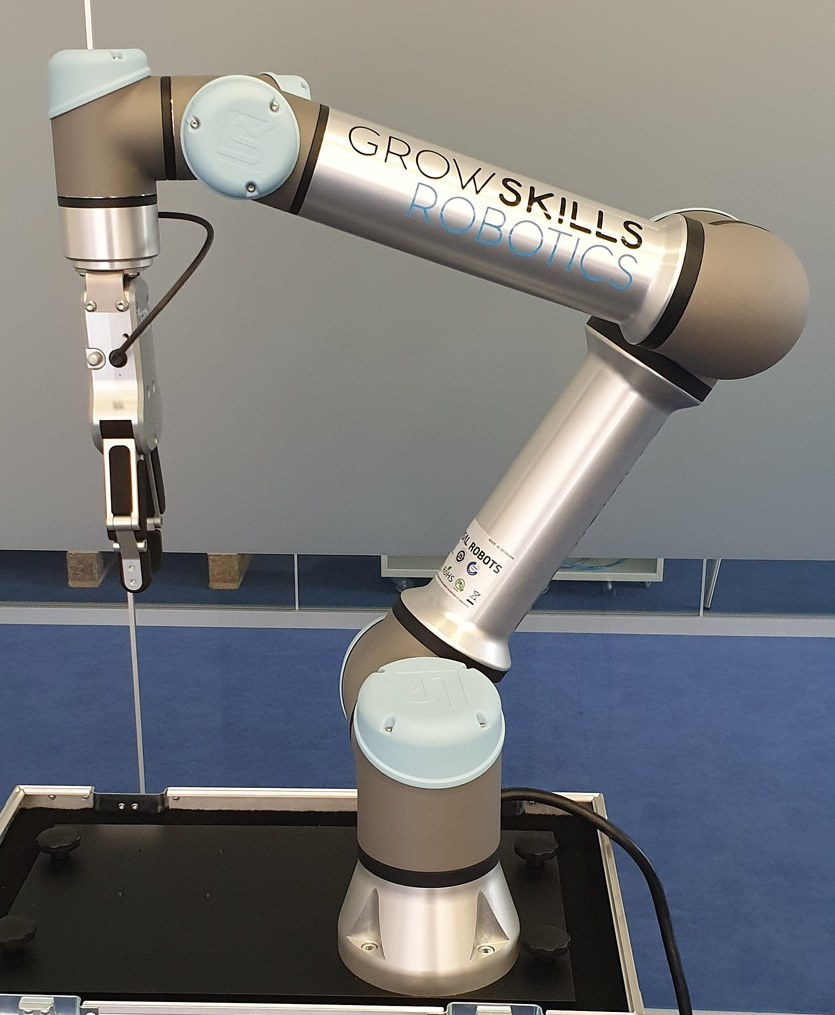
\includegraphics[height=2.3cm]{../../figures/r14_cobot.jpg}\\
\credit{GrowSkills Robotics, CC BY-SA 4.0, via Wikimedia Commons (cropped)}
\end{column}
\end{columns}
\end{frame}

% --------------------------------------------------------------------
\begin{frame}{Session 2.9 --- Check your understanding}
\begin{keybox}[Check your understanding]
\begin{enumerate}\setlength\itemsep{2mm}
\item An arm under plain PD control sags 2$^\circ$ below the target when held horizontal, but not when pointing straight up. Why?
\item Why is independent-joint PID good enough for a robot with 100:1 gearboxes, but not for a direct-drive arm?
\item A robot must wipe a table with a sponge. Would you use stiff position control or impedance control? Why?
\end{enumerate}
\end{keybox}
\vspace{2mm}
{\small\color{mkGray}Discuss in pairs for 2 minutes, then we compare answers.}
\end{frame}

% --------------------------------------------------------------------
\begin{frame}{Session 2.9 --- Summary and key terms}
\begin{columns}[T]
\begin{column}{.52\textwidth}
\begin{keybox}[Key take-aways]
\begin{itemize}\setlength\itemsep{.4mm}
\item Robot joints are coupled; inertia and gravity change with the pose.
\item Independent-joint PID + high gear ratio: the industrial standard.
\item Gravity compensation removes sag without waiting for I-action.
\item Computed torque cancels the dynamics with a model.
\item Impedance control makes contact safe and predictable.
\end{itemize}
\end{keybox}
\end{column}
\begin{column}{.46\textwidth}
\begin{defbox}[Key terms]
\small
\term{independent-joint control} one SISO loop per joint $\cdot$ \term{coupling} motion of one joint loads another $\cdot$ \term{gravity compensation} feed the modelled weight torque $\cdot$ \term{computed torque} model-based cancellation of dynamics $\cdot$ \term{impedance} chosen spring--damper behaviour $\cdot$ \term{force control} regulate contact force
\end{defbox}
\end{column}
\end{columns}
\end{frame}

% ####################################################################
\section{3.1 Servo System Architecture and Control Modes}
% ####################################################################

\begin{frame}{What is a servo system?}
\begin{columns}[T]
\begin{column}{.55\textwidth}
\small
A \term{servo} (from Latin \emph{servus}, servant) is a motor system that \hl{obeys a command} using feedback: ``go to $90^\circ$'', ``turn at 1000\,rpm'', ``push with 5\,N\,m''.
\begin{itemize}\setlength\itemsep{.4mm}
\item \term{servo motor}: usually a PMSM with an encoder and brake
\item \term{servo drive}: power electronics + control loops + protection
\item \term{motion controller}: plans the moves for all axes
\end{itemize}
\textbf{Picture:} a taxi --- the passenger (controller) says where to go, the driver (drive) handles pedals and steering, the engine (motor) does the work.
\end{column}
\begin{column}{.43\textwidth}
\centering
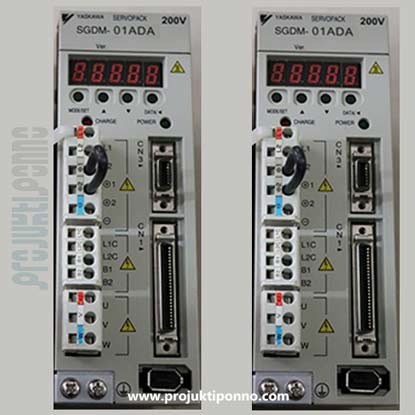
\includegraphics[width=.75\linewidth]{../../figures/d3_servo_drive_motor.jpg}\\
\credit{Projuktiponno, CC BY-SA 4.0, via Wikimedia Commons}\\
{\scriptsize industrial servo drive and motor}
\end{column}
\end{columns}
\end{frame}

% --------------------------------------------------------------------
\begin{frame}{Servo system architecture: from mains to load}
\begin{columns}[T]
\begin{column}{.68\textwidth}
\centering
\vspace{-2mm}\resizebox{\linewidth}{!}{\begin{tikzpicture}[node distance=4mm]
  \node[blk,minimum height=9mm] (Mains) {mains\\3$\sim$ 400\,V};
  \node[blk,right=of Mains,minimum height=9mm] (PS) {power\\supply};
  \node[blk,right=5mm of PS,minimum width=22mm,minimum height=19mm,fill=mkLight,anchor=west,yshift=-3mm] (Dr) {};
  \node[font=\tiny\bfseries,text=mkBlue,anchor=north] at (Dr.north) {servo drive};
  \node[blkO,font=\tiny,minimum height=4mm,anchor=north] (Ctl) at ($(Dr.north)+(0,-3.6mm)$) {pos./vel./current ctrl};
  \node[blk,font=\tiny,minimum height=4mm,below=1mm of Ctl] (Inv) {DC bus + inverter};
  \node[blk,right=6mm of Dr.east,anchor=west,minimum height=9mm,yshift=3mm] (M) {motor};
  \node[blk,right=of M,minimum height=9mm] (Tr) {gearbox\\\tiny harmonic / planetary};
  \node[blk,right=of Tr,minimum height=9mm] (L) {link +\\payload};
  \node[blkO,below=5mm of M,minimum height=5mm] (Enc) {feedback\\\tiny encoder};
  \node[blk,above=5mm of Dr,minimum height=6mm] (MC) {robot / motion controller};
  \draw[sig,line width=1pt] (Mains) -- (PS);
  \draw[sig,line width=1pt] (PS) -- (PS -| Dr.west) node[pos=.5,above,font=\tiny]{DC};
  \draw[sig,line width=1pt,mkOrange] (Dr.east |- M) -- (M) node[pos=.4,above,font=\tiny,text=mkNavy]{U V W};
  \draw[line width=1.2pt,mkNavy] (M) -- (Tr);
  \draw[line width=1.2pt,mkNavy] (Tr) -- (L);
  \draw[mkNavy,densely dotted] (M) -- (Enc);
  \draw[sig,mkMid] (Enc) -| ($(Dr.south east)+(-3mm,0)$);
  \draw[sig,mkMid,{Latex[length=1.5mm]}-{Latex[length=1.5mm]}] (MC) -- (Dr) node[pos=.5,right,font=\tiny]{fieldbus (EtherCAT \dots)};
\end{tikzpicture}}
\vspace{2mm}

\small
\begin{itemize}\setlength\itemsep{.3mm}
\item the \term{motion controller} sends targets every 0.25--4\,ms
\item the \term{drive} closes the fast loops (up to 32\,kHz)
\item the \term{encoder} closes every loop
\end{itemize}
\end{column}
\begin{column}{.30\textwidth}
\centering
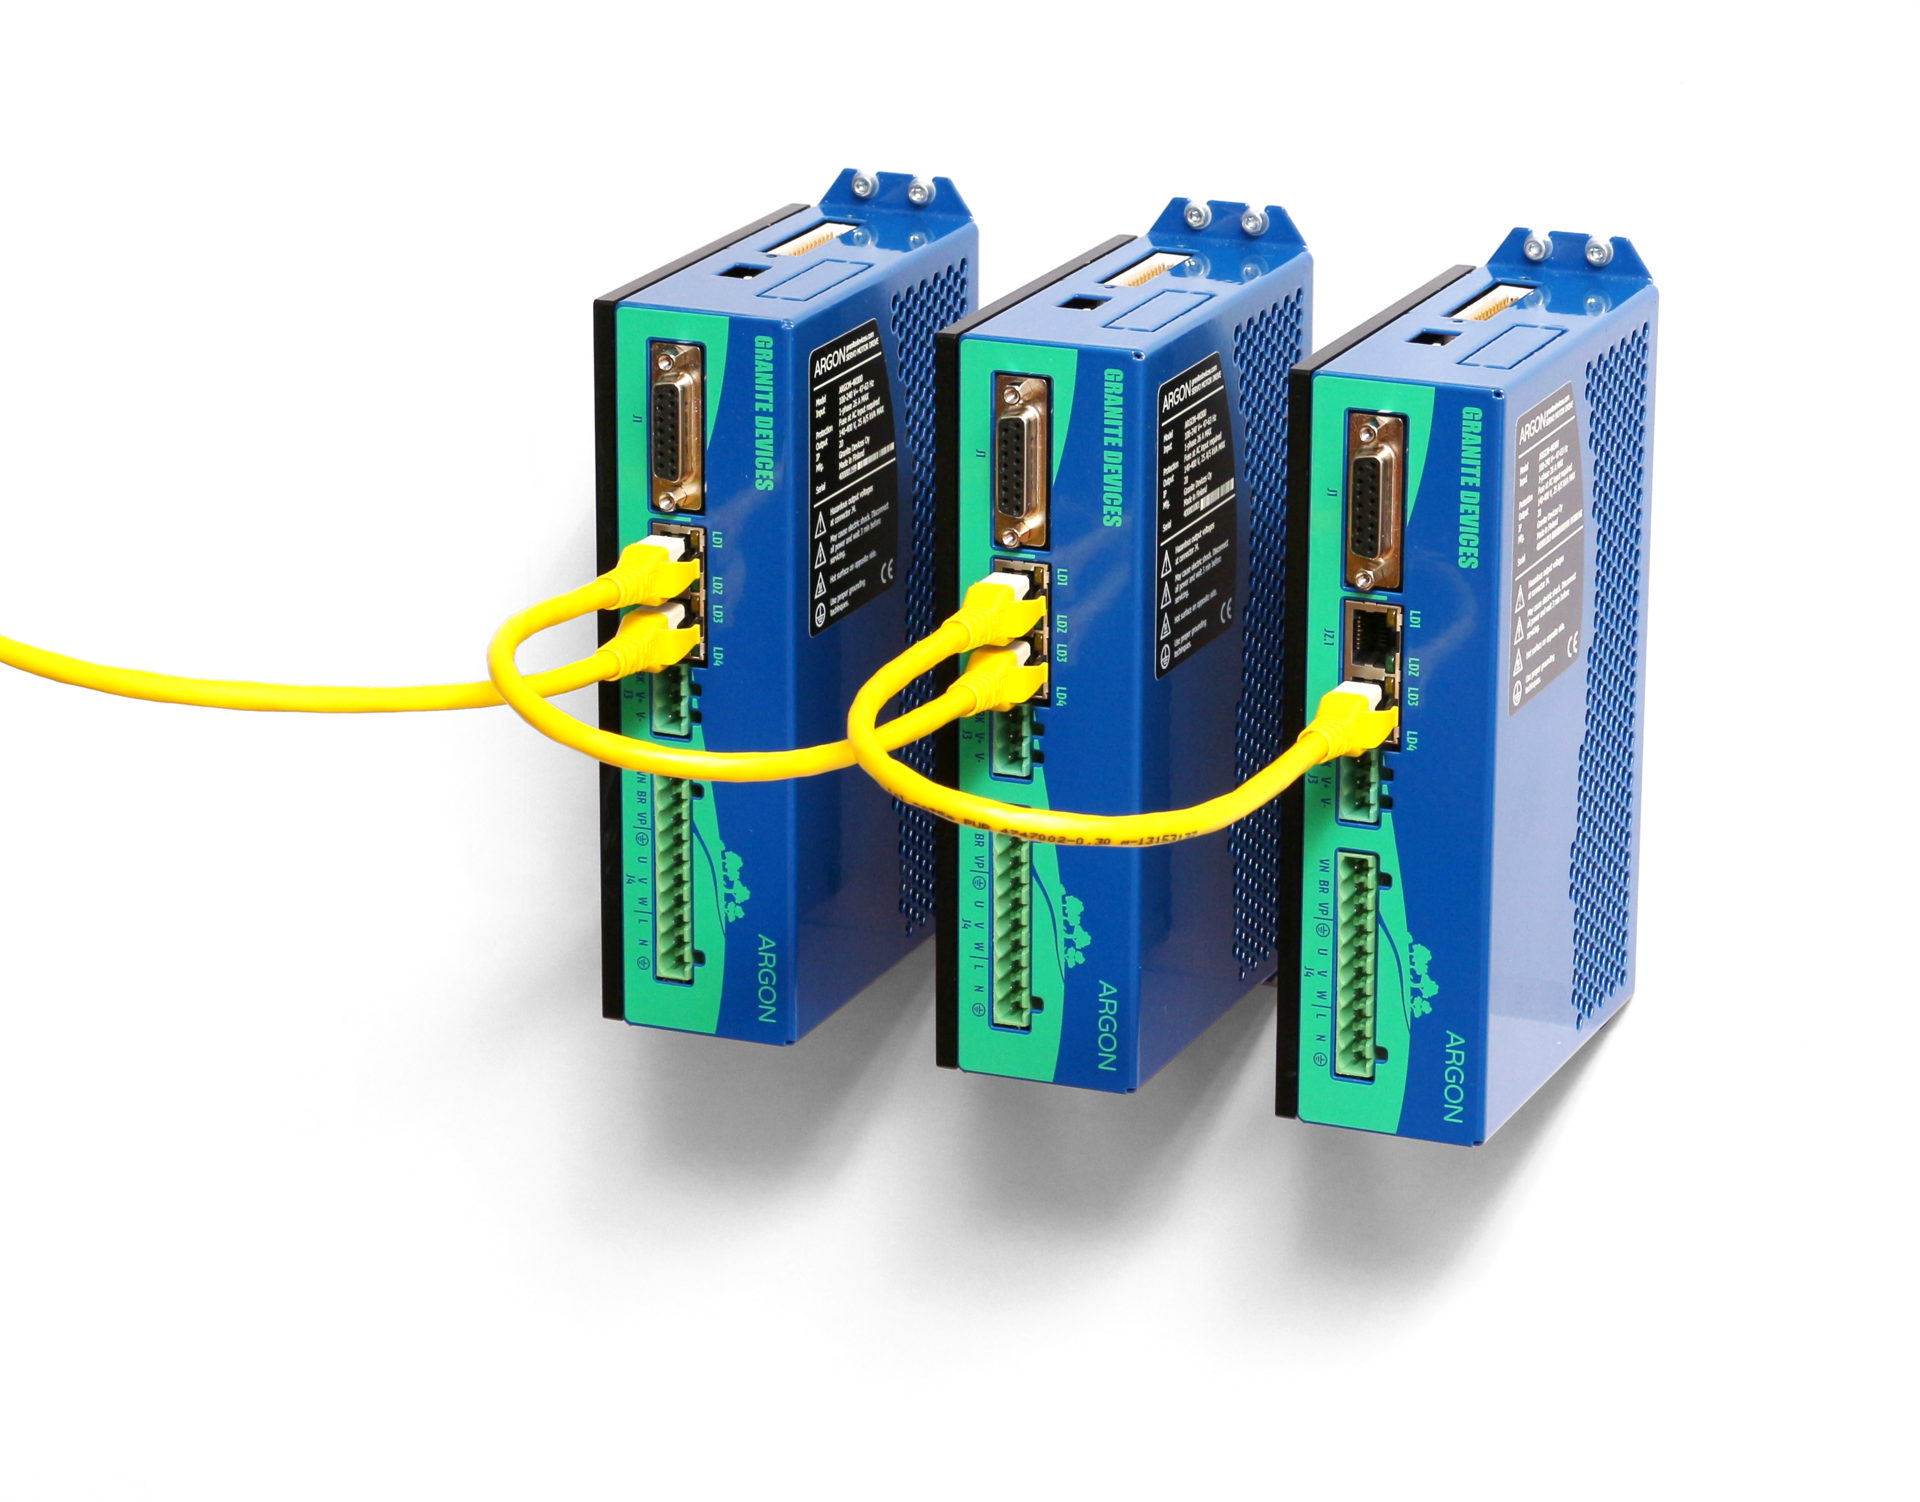
\includegraphics[width=.9\linewidth]{../../figures/d3_servo_drives.png}\\
\credit{Tero Kontkanen, CC BY-SA 3.0, via Wikimedia Commons}\\
{\scriptsize compact servo drives sharing a DC bus and a fieldbus}
\end{column}
\end{columns}
\end{frame}

% --------------------------------------------------------------------
\begin{frame}{Inside a robot joint: one servo axis per joint}
\begin{columns}[T]
\begin{column}{.58\textwidth}
\centering
\begin{tikzpicture}[scale=.95]
  % housing
  \draw[mkGray,thick,fill=mkLight] (0,0) rectangle (7.0,2.0);
  \draw[mkBlue,thick,fill=mkPale] (0.2,0.3) rectangle (1.2,1.7); \node[font=\tiny,align=center] at (0.7,1.0) {encoder};
  \draw[mkBlue,thick,fill=mkPale] (1.3,0.3) rectangle (2.2,1.7); \node[font=\tiny,align=center] at (1.75,1.0) {brake};
  \draw[mkOrange,thick,fill=mkCream] (2.3,0.2) rectangle (4.3,1.8); \node[font=\tiny,align=center] at (3.3,1.0) {PMSM\\motor};
  \draw[mkBlue,thick,fill=mkPale] (4.4,0.3) rectangle (5.8,1.7); \node[font=\tiny,align=center] at (5.1,1.0) {harmonic\\gearbox};
  \draw[mkNavy,thick,fill=mkSky] (5.9,0.5) rectangle (6.8,1.5); \node[font=\tiny,align=center] at (6.35,1.0) {output\\flange};
  \draw[mkNavy,thick,fill=white] (6.9,1.0) -- (7.6,1.0);
  \draw[line width=5pt,mkBlue,line cap=round] (7.6,1.0) -- (8.4,2.0);
  \node[font=\tiny,anchor=west] at (7.7,2.15) {next link};
  \node[font=\tiny,text=mkGray,anchor=north] at (3.5,-0.05) {joint housing (often with an integrated drive)};
  \draw[mkMid,thick,-{Latex[length=1.4mm]}] (3.3,-0.6) -- (3.3,-0.3);
  \node[font=\tiny,text=mkMid,anchor=north] at (3.3,-0.6) {power + EtherCAT cable through the arm};
\end{tikzpicture}

\vspace{1mm}
\small
\begin{itemize}\setlength\itemsep{.3mm}
\item a 6-axis robot = \hl{six servo axes} coordinated by one controller
\item the \term{holding brake} keeps the arm up when power is off
\item gearbox ratio 50--160 (W1D2)
\end{itemize}
\end{column}
\begin{column}{.40\textwidth}
\centering
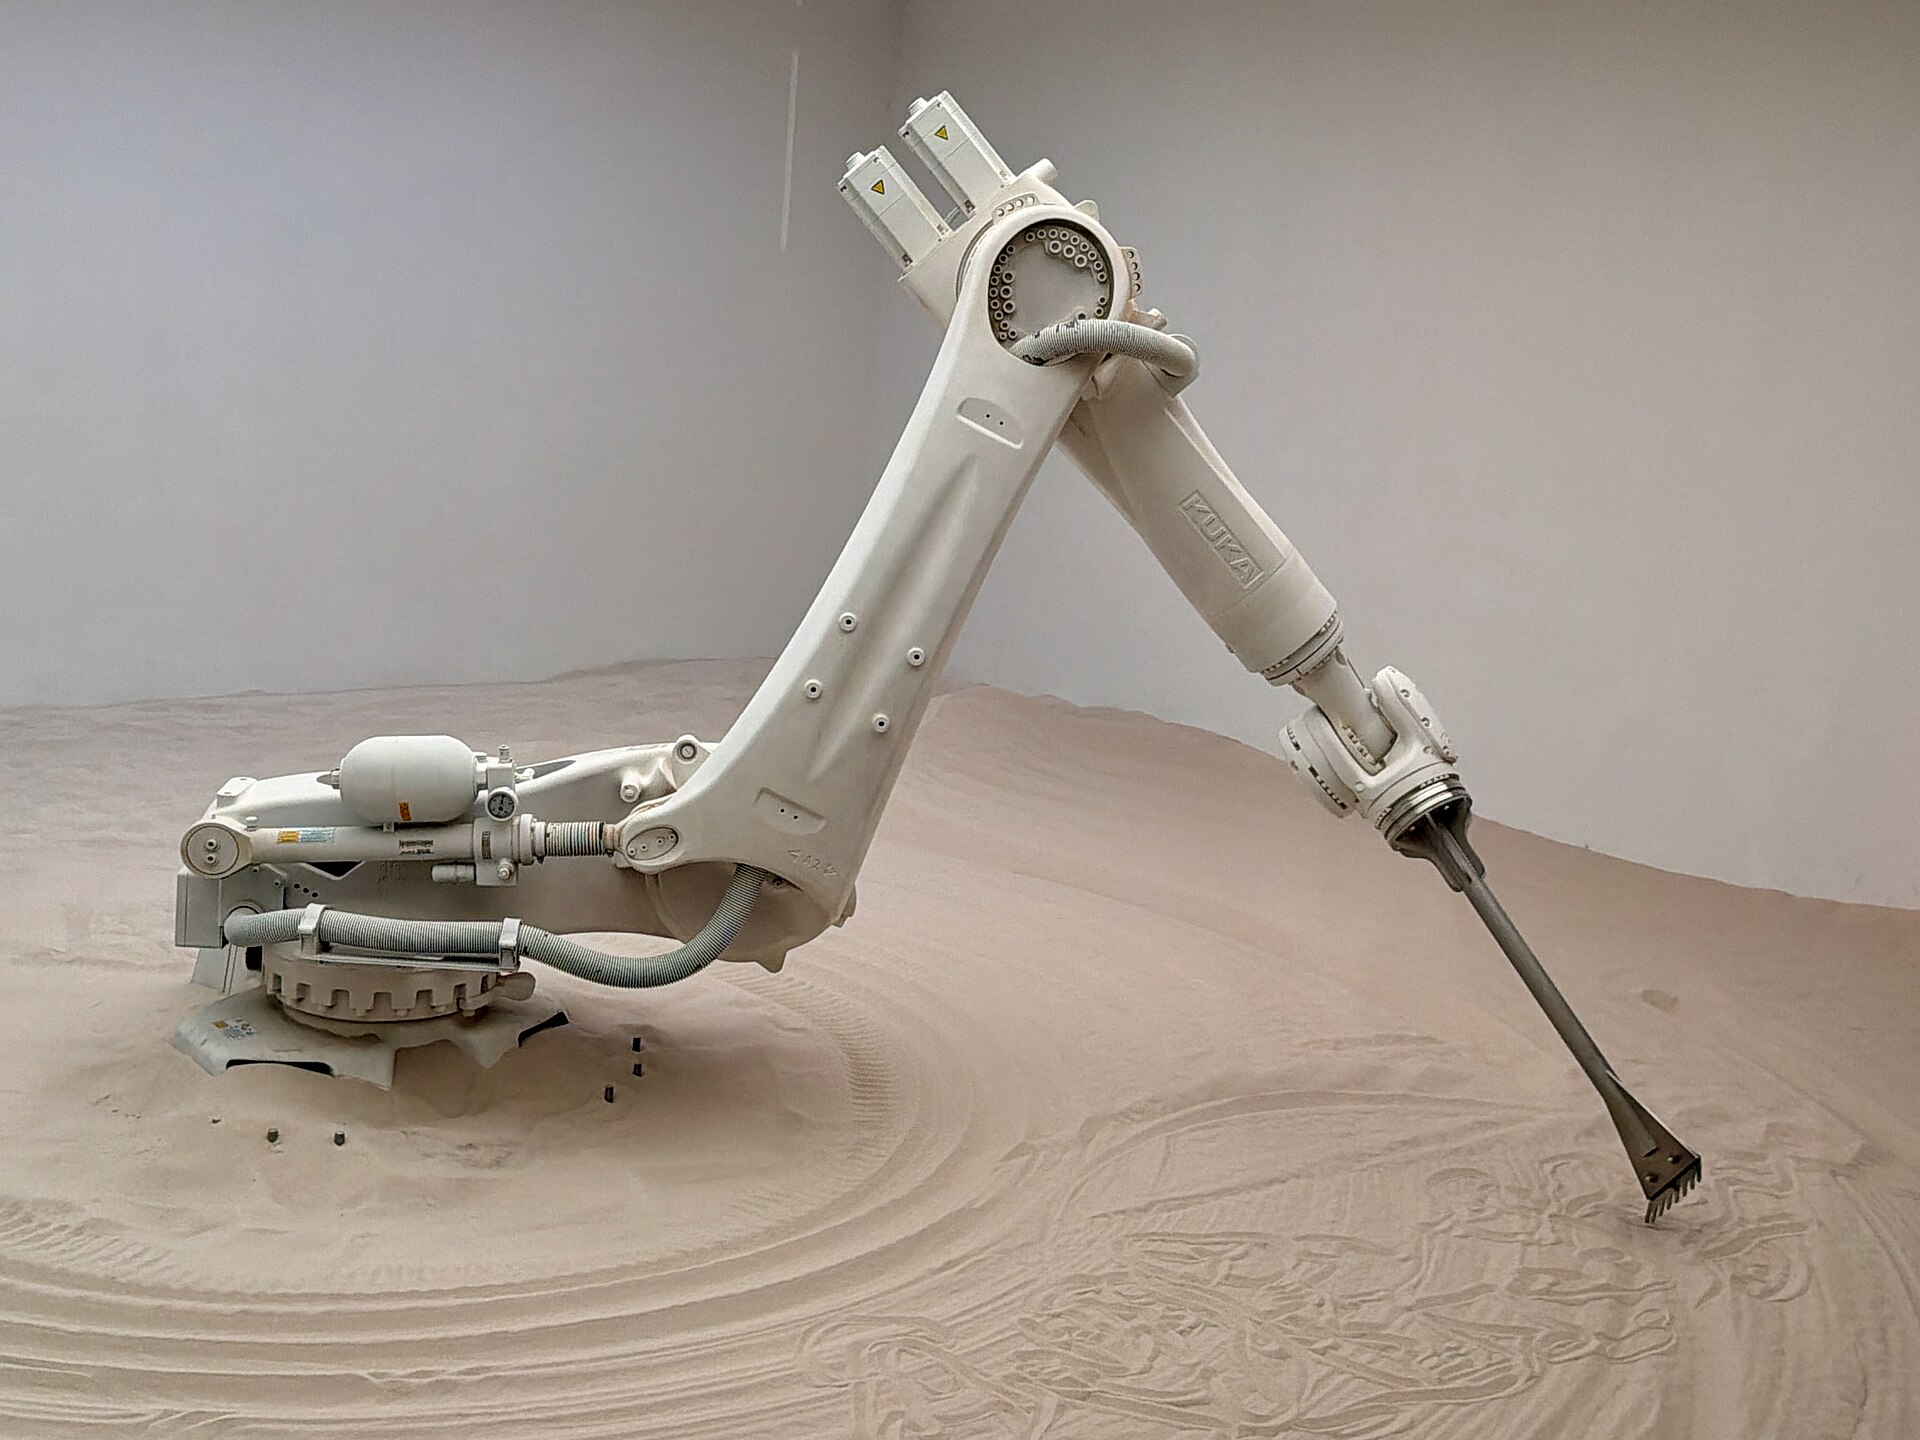
\includegraphics[width=.95\linewidth]{../../figures/d4_kuka_robot.jpg}\\
\credit{Oleg Yunakov, CC BY-SA 4.0, via Wikimedia Commons}\\[1mm]
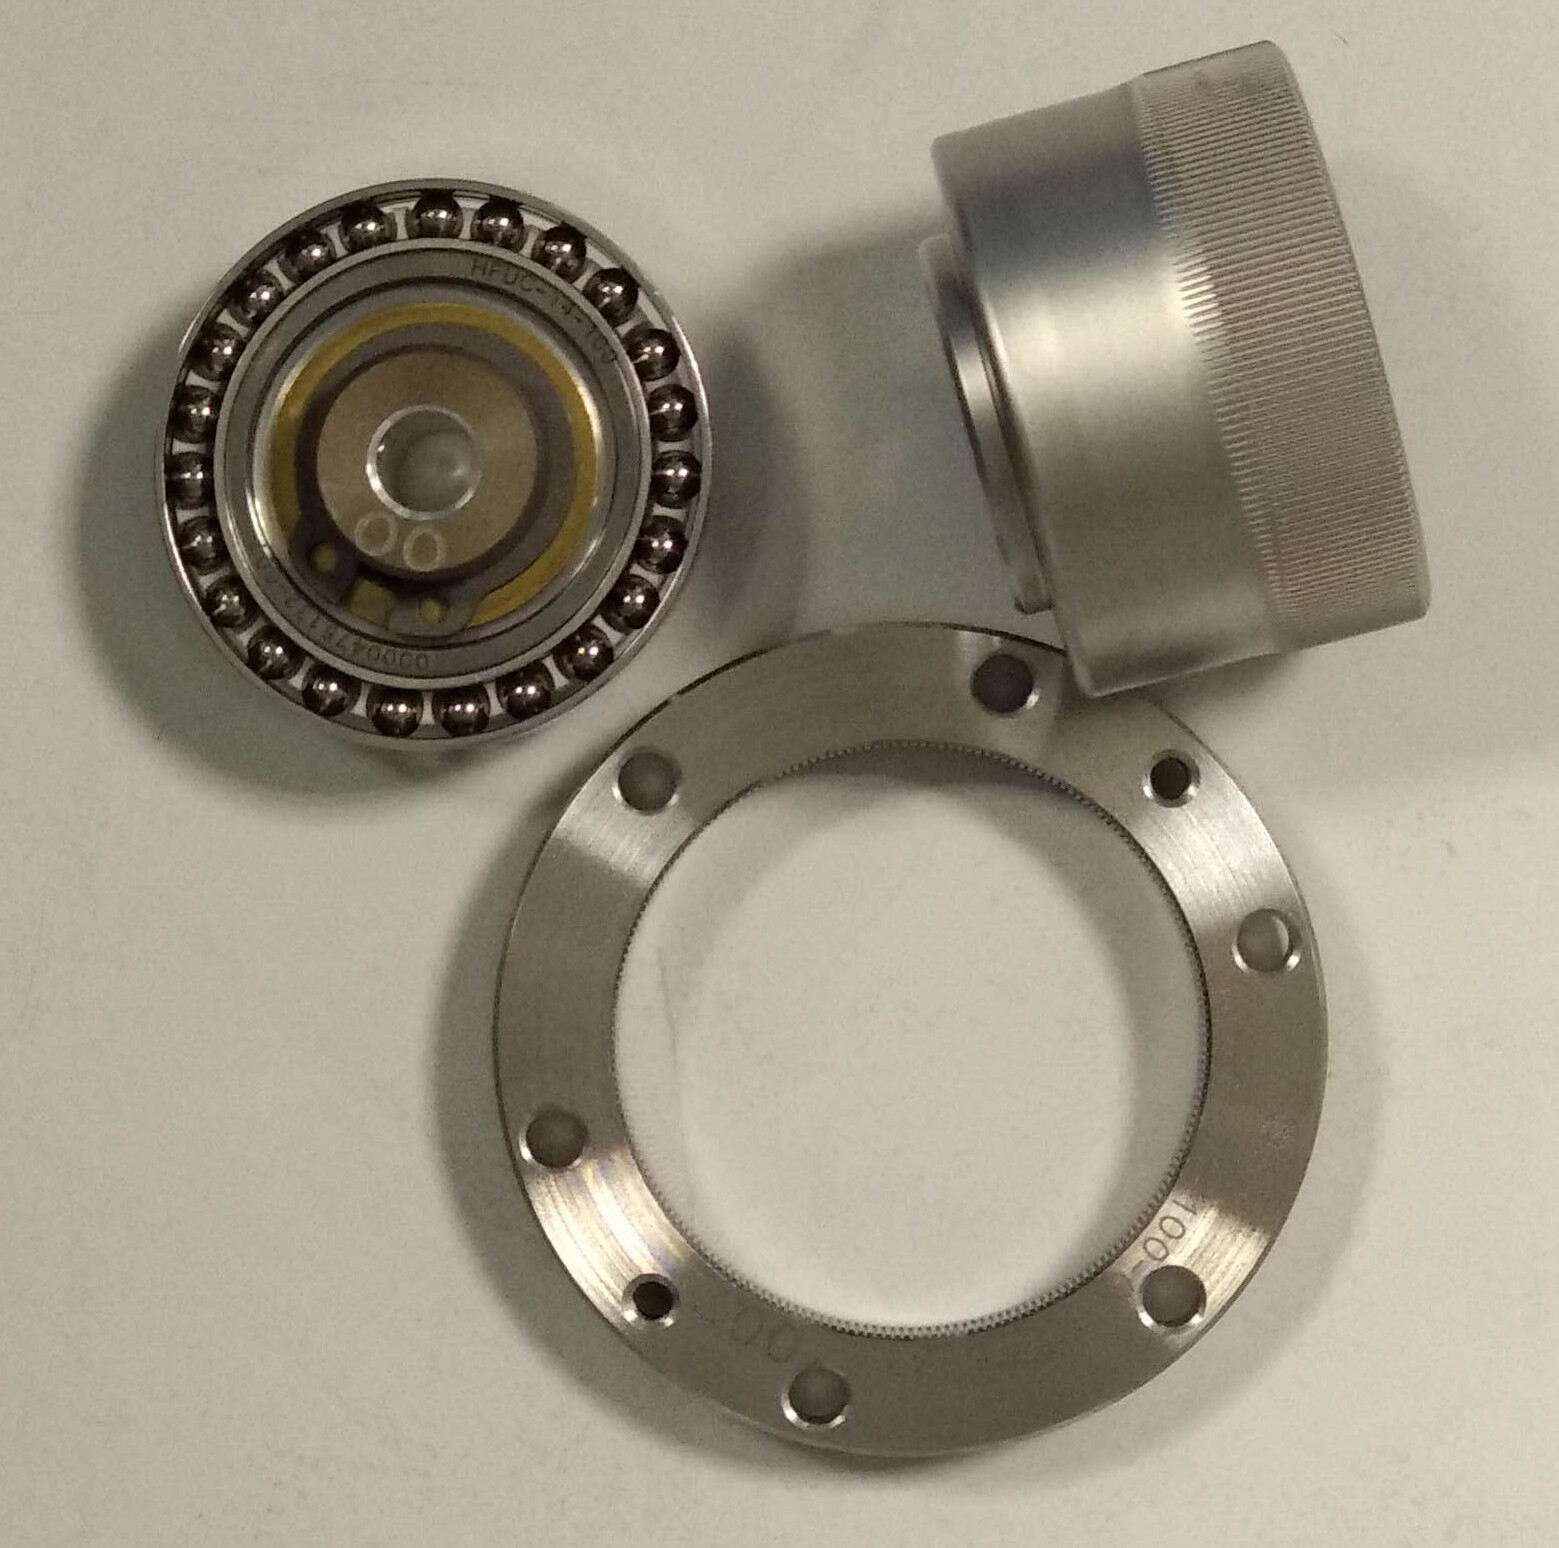
\includegraphics[height=1.7cm]{../../figures/d1_harmonic_drive.jpg}\\
\credit{Pieceofmetalwork, CC BY-SA 4.0, via Wikimedia Commons}
\end{column}
\end{columns}
\end{frame}

% --------------------------------------------------------------------
\begin{frame}{Torque, velocity and position control modes}
\small
\begin{tabularx}{\textwidth}{@{}l >{\raggedright\arraybackslash}X >{\raggedright\arraybackslash}X l >{\raggedright\arraybackslash}X@{}}
\toprule
\textbf{Mode} & \textbf{Controller sends} & \textbf{Loops in the drive} & \textbf{Typ.\ BW} & \textbf{Robotics example}\\
\midrule
Torque & torque $T^*$ & current only & 1--3\,kHz & computed torque, force/impedance control, cobots\\
Velocity & speed $\omega^*$ & velocity + current & 100--500\,Hz & AMR wheels, conveyor tracking\\
Position & angle $\theta^*$ & position + velocity + current & 20--100\,Hz & industrial arm joints, gantries\\
\bottomrule
\end{tabularx}
\vspace{3mm}
\begin{columns}[T]
\begin{column}{.52\textwidth}
\small
\textbf{Analogy:} telling a driver ``press the pedal this much'' (torque), ``drive at 50\,km/h'' (velocity) or ``stop at that line'' (position).
\vspace{1mm}

{\scriptsize\color{mkGray}Going further: fieldbus drive profiles (CiA\,402) call these CST, CSV, CSP --- W2D5.}
\end{column}
\begin{column}{.46\textwidth}
\begin{keybox}[Selection rule]
Close each loop where its \textbf{sensor} is and where it can be updated \textbf{fast enough}. Model-based robot control (2.9) needs \hl{torque mode}.
\end{keybox}
\end{column}
\end{columns}
\end{frame}

% --------------------------------------------------------------------
\begin{frame}{Cascade control structure of a servo drive}
\centering
\resizebox{\linewidth}{!}{\begin{tikzpicture}[node distance=4.5mm]
  \node[sumn] (Sp) {\sumsym};
  \node[blk,right=of Sp] (Cp) {$K_{pp}$\\[-.5mm]\tiny position P};
  \node[sumn,right=6mm of Cp] (Sv) {\sumsym};
  \node[blk,right=of Sv] (Cv) {PI\\[-.5mm]\tiny velocity};
  \node[sumn,right=6mm of Cv] (Si) {\sumsym};
  \node[blk,right=of Si] (Ci) {PI\\[-.5mm]\tiny current};
  \node[blkO,right=of Ci] (Inv) {PWM\\inverter};
  \node[blk,right=of Inv] (Mot) {$\frac{1}{Ls+R}$\\[-.5mm]\tiny winding};
  \node[blk,right=of Mot] (Kt) {$k_t$};
  \node[blk,right=of Kt] (Mech) {$\frac{1}{Js}$};
  \node[blk,right=of Mech] (Int) {$\frac1s$};
  \draw[sig] ($(Sp.west)+(-5mm,0)$) node[left,font=\scriptsize]{$\theta^*$} -- (Sp);
  \draw[sig] (Sp) -- (Cp); \draw[sig] (Cp) -- (Sv); \draw[sig] (Sv) -- (Cv);
  \draw[sig] (Cv) -- (Si); \draw[sig] (Si) -- (Ci); \draw[sig] (Ci) -- (Inv);
  \draw[sig] (Inv) -- node[above,font=\tiny]{$v$} (Mot); \draw[sig] (Mot) -- node[above,font=\tiny]{$i$} (Kt);
  \draw[sig] (Kt) -- node[above,font=\tiny]{$T_m$} (Mech); \draw[sig] (Mech) -- node[above,font=\tiny]{$\omega$} (Int);
  \draw[sig] (Int.east) -- ++(4mm,0) node[right,font=\scriptsize]{$\theta$};
  \draw[sig] ($(Int.east)+(2mm,0)$) -- ++(0,-14mm) -| node[pos=.97,left,font=\tiny]{$-$} (Sp);
  \draw[sig] ($(Mech.east)!.5!(Int.west)$) -- ++(0,-9mm) -| node[pos=.95,left,font=\tiny]{$-$} (Sv);
  \draw[sig] ($(Mot.east)!.5!(Kt.west)$) -- ++(0,-4.5mm) -| node[pos=.9,left,font=\tiny]{$-$} (Si);
  \draw[sig,mkOrange,densely dashed] ($(Sp.west)+(-3mm,0)$) -- ++(0,9mm) -| node[pos=.25,above,font=\tiny,text=mkOrange]{velocity feedforward $\dot\theta^*$} (Sv.north);
  \draw[sig,mkOrange,densely dashed] ($(Sp.west)+(-3mm,9mm)$) -- ++(0,6mm) -| node[pos=.2,above,font=\tiny,text=mkOrange]{torque feedforward $\hat J\ddot\theta^*$ (+ gravity)} (Si.north);
\end{tikzpicture}}
\vspace{2mm}
\begin{columns}[T]
\begin{column}{.5\textwidth}
\small
\textbf{Picture:} Russian dolls --- each inner loop turns its part into something simple for the next one (current loop $\rightarrow$ ``ideal torque source'').
\end{column}
\begin{column}{.48\textwidth}
\small
\begin{itemize}\setlength\itemsep{.3mm}
\item each inner loop \hl{3--10$\times$} faster than the next
\item tune from inside out: current $\rightarrow$ velocity $\rightarrow$ position
\item feedforward acts on the plan before an error appears
\end{itemize}
\end{column}
\end{columns}
\src{[Ellis, 2012, ch.~17]; details and tuning in W1D5 (sessions 3.4--3.5).}
\end{frame}

% --------------------------------------------------------------------
\begin{frame}{The bandwidth hierarchy}
\begin{columns}[T]
\begin{column}{.52\textwidth}
\centering
\begin{tikzpicture}
\begin{axis}[mkplot,xmode=log,width=7.6cm,height=5.2cm,xmin=1,xmax=30000,ymin=-40,ymax=6,xlabel={$f$ [Hz]},ylabel={closed-loop $|T|$ [dB]},
   legend style={at={(0.02,0.03)},anchor=south west,font=\tiny}]
\addplot[mkMid,thick] table[x=f,y=pc]{data/bw.dat};\addlegendentry{position ($\approx40$\,Hz)}
\addplot[mkOrange,thick] table[x=f,y=vc]{data/bw.dat};\addlegendentry{velocity ($\approx250$\,Hz)}
\addplot[mkBlue,thick] table[x=f,y=ic]{data/bw.dat};\addlegendentry{current ($\approx2$\,kHz)}
\draw[mkGray,densely dashed] (axis cs:1,-3) -- (axis cs:30000,-3);
\end{axis}
\end{tikzpicture}
\end{column}
\begin{column}{.46\textwidth}
\small
\textbf{Bandwidth} = how fast a loop can follow its command (the $-3$\,dB point).
\begin{itemize}\setlength\itemsep{.4mm}
\item current $\approx$ 2\,kHz: limited by PWM and sampling
\item velocity $\approx$ 250\,Hz: limited by inertia, resonances, encoder noise
\item position $\approx$ 40\,Hz: limited by the velocity loop
\end{itemize}
\begin{keybox}[Take-away]
Separate the loops by \hl{3--10$\times$} so each outer loop sees the inner one as ``instant''.
\end{keybox}
\end{column}
\end{columns}
\end{frame}

% --------------------------------------------------------------------
\begin{frame}{Session 3.1 --- Check your understanding}
\begin{keybox}[Check your understanding]
\begin{enumerate}\setlength\itemsep{2mm}
\item A cobot controller computes joint torques from a dynamic model every 1\,ms. Which drive mode should the joints run in?
\item The position loop is tuned to 300\,Hz while the velocity loop reaches only 100\,Hz. What goes wrong?
\item Why must the current loop be tuned first?
\end{enumerate}
\end{keybox}
\vspace{2mm}
{\small\color{mkGray}Discuss in pairs for 2 minutes, then we compare answers.}
\end{frame}

% --------------------------------------------------------------------
\begin{frame}{Session 3.1 --- Summary and key terms}
\begin{columns}[T]
\begin{column}{.52\textwidth}
\begin{keybox}[Key take-aways]
\begin{itemize}\setlength\itemsep{.4mm}
\item Servo = supply + drive + motor + gearbox + load + encoder + controller.
\item A robot joint is one complete servo axis.
\item Mode = which loops the drive closes (torque / velocity / position).
\item Cascade: current $\gg$ velocity $\gg$ position bandwidth.
\end{itemize}
\end{keybox}
\end{column}
\begin{column}{.46\textwidth}
\begin{defbox}[Key terms]
\small
\term{servo drive} power stage + loops $\cdot$ \term{motion controller} plans the moves $\cdot$ \term{control mode} torque, velocity or position $\cdot$ \term{cascade} loops inside loops $\cdot$ \term{feedforward} act on the reference $\cdot$ \term{bandwidth} how fast a loop follows
\end{defbox}
\end{column}
\end{columns}
\end{frame}

% ####################################################################
\section{3.2 Power Electronics for Drives}
% ####################################################################

\begin{frame}{Refresher: diode, capacitor and transistor switch}
\begin{columns}[T]
\begin{column}{.32\textwidth}
\centering
\begin{circuitikz}[scale=.8,transform shape]
\draw (0,0) to[D*,l=$D$] (2.2,0);
\end{circuitikz}
\begin{defbox}[Diode]
\small
A one-way \term{valve}: current flows only from anode to cathode. Turns AC into DC (rectifier).
\end{defbox}
\end{column}
\begin{column}{.32\textwidth}
\centering
\begin{circuitikz}[scale=.8,transform shape]
\draw (0,0) to[eC,l=$C$] (2.2,0);
\end{circuitikz}
\begin{defbox}[Capacitor]
\small
An energy \term{tank}: smooths the voltage and buffers bursts of current.
\[ E=\tfrac12CV^2 \]
\end{defbox}
\end{column}
\begin{column}{.32\textwidth}
\centering
\begin{circuitikz}[scale=.8,transform shape]
\draw (0,0) node[nigbt,rotate=90](T){};
\node[font=\scriptsize,anchor=north] at (T.G) {gate};
\end{circuitikz}
\begin{defbox}[Transistor switch]
\small
A tap opened by a small \term{gate} signal. Used only fully \hl{on} or fully \hl{off}.
\end{defbox}
\end{column}
\end{columns}
\vspace{1mm}
\small
\textbf{Why only on/off?} Power loss $P=V\cdot I$ in the switch. At $I=\SI{10}{A}$:
on: $V\approx\SI{1.5}{V}\Rightarrow\SI{15}{W}$; off: $I\approx0\Rightarrow\SI{0}{W}$; half-way ($V=\SI{280}{V}$): \hl{2.8\,kW} --- it would melt.
\begin{keybox}[Take-away]
A drive builds any voltage by switching very fast between on and off and averaging (PWM).
\end{keybox}
\end{frame}

% --------------------------------------------------------------------
\begin{frame}{Power stage of a servo drive: overview}
\centering
\resizebox{.92\linewidth}{!}{%
\begin{circuitikz}[scale=1,transform shape,line width=.6pt]
\ctikzset{bipoles/length=.85cm,diodes/scale=.8}
\draw (1,3) -- (2.9,3); \draw (1,0) -- (11.4,0);
\foreach \x in {1,1.8,2.6}{
  \draw (\x,1.85) to[D*] (\x,3);
  \draw (\x,0) to[D*] (\x,1.15);
  \draw (\x,1.15) -- (\x,1.85);
}
\draw (1,3) -- (2.6,3);
\draw (-0.3,1.7) node[ocirc,label={[font=\scriptsize]left:L1}]{} -- (1,1.7) node[circ]{};
\draw (-0.3,1.5) node[ocirc,label={[font=\scriptsize]left:L2}]{} -- (1.8,1.5) node[circ]{};
\draw (-0.3,1.3) node[ocirc,label={[font=\scriptsize]left:L3}]{} -- (2.6,1.3) node[circ]{};
\node[font=\scriptsize,text=mkBlue] at (1.8,3.55) {diode rectifier};
\draw (2.6,3) -- (3.0,3) to[R,l=\scriptsize$R_{pc}$] (4.4,3) -- (4.8,3);
\draw (3.0,3) -- (3.0,3.7) to[nos,l=\scriptsize bypass] (4.4,3.7) -- (4.4,3);
\draw (4.8,3) -- (5.4,3) to[eC,l_=\scriptsize$C_{dc}$] (5.4,0);
\draw (5.0,2.6) node[font=\scriptsize,text=mkOrange]{$+$};
\draw[mkOrange,-{Latex[length=1.6mm]}] (4.75,0.4) -- (4.75,2.4) node[midway,left,font=\scriptsize,text=mkOrange]{$V_{dc}$};
\draw (5.4,3) -- (6.6,3) to[R,l=\scriptsize$R_b$] (6.6,1.7);
\draw (6.6,1.7) node[nigbt,anchor=C,scale=.8](Tb){};
\draw (Tb.E) -- (6.6,0);
\node[font=\scriptsize,text=mkBlue] at (6.6,3.55) {brake chopper};
\draw (6.6,3) -- (10.6,3);
\foreach \x/\n in {8.0/a,9.3/b,10.6/c}{
  \draw (\x,3) node[nigbt,anchor=C,scale=.8](T\n u){};
  \draw (T\n u.E) -- (\x,1.35);
  \draw (\x,1.35) node[nigbt,anchor=C,scale=.8](T\n l){};
  \draw (T\n l.E) -- (\x,0);
  \draw (T\n u.C) -- ++(0.45,0) to[D*,diodes/scale=.6] ($(T\n u.E)+(0.45,0)$) -- (T\n u.E);
  \draw (T\n l.C) -- ++(0.45,0) to[D*,diodes/scale=.6] ($(T\n l.E)+(0.45,0)$) -- (T\n l.E);
}
\node[font=\scriptsize,text=mkBlue] at (9.3,3.55) {three-phase inverter};
\coordinate (ua) at (8.0,1.75); \coordinate (ub) at (9.3,1.6); \coordinate (uc) at (10.6,1.45);
\draw (ua) node[circ]{} -- (11.9,1.75); \draw (ub) node[circ]{} -- (11.9,1.6); \draw (uc) node[circ]{} -- (11.9,1.45);
\draw[fill=mkPale,draw=mkBlue,thick] (12.45,1.6) circle (0.5) node[font=\small]{M};
\node[font=\tiny] at (11.75,1.95) {U V W};
\end{circuitikz}}
\vspace{1mm}

\small
\begin{itemize}\setlength\itemsep{.3mm}
\item \textbf{AC $\rightarrow$ DC $\rightarrow$ AC}: diodes rectify the mains, the capacitor holds a steady \term{DC bus}
\item six transistor switches chop it into motor voltages of any amplitude and frequency
\item the \term{brake chopper} burns surplus energy when the motor brakes
\end{itemize}
\end{frame}

% --------------------------------------------------------------------
\begin{frame}{Rectifier and DC bus}
\begin{columns}[T]
\begin{column}{.5\textwidth}
\centering
\begin{tikzpicture}
\begin{axis}[mkplot,width=7.3cm,height=4.6cm,xmin=0,xmax=40,ymin=-600,ymax=650,xlabel={$t$ [ms]},ylabel={[V]},
  ytick={-565,0,540,565},yticklabels={$-566$,0,540,566},legend style={at={(0.98,0.03)},anchor=south east,font=\tiny}]
\foreach \c in {ab,bc,ca,ba,cb,ac} {\addplot[mkSky,thin,forget plot] table[x=t,y=\c]{data/rect.dat};}
\addplot[mkOrange,very thick] table[x=t,y=dc]{data/rect.dat};\addlegendentry{$v_{dc}$ (no capacitor)}
\draw[mkBlue,densely dashed] (axis cs:0,540) -- (axis cs:40,540);
\end{axis}
\end{tikzpicture}
\small
The diodes always pick the highest of the six line-to-line voltages: a bumpy DC.
\end{column}
\begin{column}{.48\textwidth}
\small
\begin{eqbox}
\[ V_{dc}\approx1.35\,V_{LL}\ \text{(average)},\quad \hat V=\sqrt2\,V_{LL} \]
\end{eqbox}
\textbf{Example:} 400\,V mains: $1.35\times400=\SI{540}{V}$; with a capacitor it charges to the peak $\sqrt2\cdot400\approx\SI{566}{V}$.
\begin{itemize}\setlength\itemsep{.3mm}
\item $C_{dc}$ smooths the bumps
\item pre-charge resistor limits the inrush into an empty $C_{dc}$
\item diodes cannot send energy \hl{back} to the mains
\item small robots and AMRs: a 24--48\,V battery \emph{is} the DC bus
\end{itemize}
\end{column}
\end{columns}
\end{frame}

% --------------------------------------------------------------------
\begin{frame}{PWM: duty cycle and average voltage}
\begin{columns}[T]
\begin{column}{.52\textwidth}
\centering
\begin{tikzpicture}[x=.95cm,y=1.0cm]
  \draw[-{Latex[length=2mm]},mkGray] (0,0) -- (6.3,0) node[right,font=\scriptsize]{$t$};
  \draw[-{Latex[length=2mm]},mkGray] (0,0) -- (0,2.4) node[above,font=\scriptsize]{$v$};
  \foreach \k in {0,1,2}{
    \draw[mkBlue,line width=1pt] (2*\k,0) -- (2*\k,2) -- (2*\k+.8,2) -- (2*\k+.8,0) -- (2*\k+2,0);
  }
  \draw[mkOrange,line width=1.1pt,dashed] (0,.8) -- (6,.8) node[right,font=\scriptsize]{$\bar v=D\,V_\text{dc}$};
  \node[font=\scriptsize,anchor=east] at (0,2) {$V_\text{dc}$};
  \draw[|-|,mkMid] (0,2.25) -- node[above,font=\tiny]{$t_\text{on}$} (.8,2.25);
  \draw[|-|,mkGray] (2,-.35) -- node[below,font=\tiny]{period $T_{sw}$} (4,-.35);
\end{tikzpicture}\\[3mm]
\small \textbf{Analogy:} flick a light switch on and off very fast --- the room looks evenly \emph{dimmed}. The motor inductance smooths the current pulses like a flywheel.
\end{column}
\begin{column}{.46\textwidth}
\small
\begin{itemize}\setlength\itemsep{.4mm}
\item \term{PWM} (pulse-width modulation): switch fully on/off at a fixed rate, vary the on-time
\item \term{duty cycle} $D=t_\text{on}/T_{sw}$ (0 \ldots 1)
\end{itemize}
\begin{eqbox}
\[ \bar v = D\cdot V_\text{dc} \]
\end{eqbox}
\textbf{Example:} $V_\text{dc}=\SI{48}{V}$ (robot joint), $f_{sw}=\SI{20}{kHz}$ ($T_{sw}=\SI{50}{\micro s}$), $t_\text{on}=\SI{15}{\micro s}$:
\begin{enumerate}\setlength\itemsep{.2mm}
\item $D=15/50=0.3$
\item $\bar v=0.3\cdot48=\SI{14.4}{V}$
\end{enumerate}
\end{column}
\end{columns}
\end{frame}

% --------------------------------------------------------------------
\begin{frame}{Three-phase inverter and sinusoidal PWM}
\begin{columns}[T]
\begin{column}{.38\textwidth}
\centering
\begin{circuitikz}[scale=.7,transform shape,line width=.5pt]
\draw (0,0) -- (6,0);  \draw (0,4) -- (6,4);
\draw (0,4) to[C,l_=$C_\text{dc}$] (0,0);
\node[anchor=east,font=\scriptsize] at (-.4,2.0) {$V_\text{dc}$};
\foreach \x/\n in {1.6/a,3.4/b,5.2/c}{
  \draw (\x,4) to[Tnigbt,mirror] (\x,2) to[Tnigbt,mirror] (\x,0);
  \draw (\x,2) to[short,*-o] (\x+.6,2) node[right,font=\scriptsize]{$\n$};
}
\end{circuitikz}\\[2mm]
\small
\begin{itemize}\setlength\itemsep{.3mm}
\item each \term{leg}: two switches, \hl{never on together}
\item compare a sine with a fast triangle
\item sine above triangle $\Rightarrow$ upper switch on
\item duty cycle follows the sine $\Rightarrow$ average voltage is a sine
\end{itemize}
\end{column}
\begin{column}{.60\textwidth}
\centering
\begin{tikzpicture}
\begin{groupplot}[group style={group size=1 by 3,vertical sep=2mm,xticklabels at=edge bottom},
  mkplot,width=8.1cm,xmin=0,xmax=360,xtick={0,90,180,270,360},
  every axis plot/.append style={line width=.5pt},grid=none,yticklabel style={font=\tiny}]
\nextgroupplot[height=2.8cm,ymin=-1.1,ymax=1.1,ylabel={sine, triangle},ytick={-1,0,1}]
\addplot[mkSky,line width=.3pt] table[x=th,y=car]{data/spwm.dat};
\addplot[mkBlue,thick] table[x=th,y=va]{data/spwm.dat};
\addplot[mkOrange,thick] table[x=th,y=vb]{data/spwm.dat};
\nextgroupplot[height=2.0cm,ymin=-.2,ymax=2.4,ytick={0.5,1.8},yticklabels={$S_a$,$S_b$}]
\addplot[mkBlue] table[x=th,y=Sa]{data/spwm.dat};
\addplot[mkOrange] table[x=th,y expr=\thisrow{Sb}+1.3]{data/spwm.dat};
\nextgroupplot[height=2.3cm,ymin=-1.3,ymax=1.3,ytick={-1,0,1},ylabel={$v_{ab}/V_\text{dc}$},xlabel={angle of the sine [$^\circ$]}]
\addplot[mkMid] table[x=th,y=vab]{data/spwm.dat};
\addplot[mkOrange,thick,domain=0:360,samples=90] {0.8*0.866*sin(x+30)};
\end{groupplot}
\end{tikzpicture}
\begin{eqbox}
\small\centering
peak phase voltage $\hat V_1=m\,\dfrac{V_\text{dc}}{2}$, \ \ $m$ = \term{modulation index} (0\ldots1)
\end{eqbox}
\end{column}
\end{columns}
\end{frame}

% --------------------------------------------------------------------
\begin{frame}{Voltage and current limits: the torque--speed envelope}
\begin{columns}[T]
\begin{column}{.52\textwidth}
\centering
\begin{tikzpicture}
\begin{axis}[mkplot,width=7.4cm,height=5.2cm,xmin=0,xmax=8000,ymin=0,ymax=16,
  xlabel={speed $n$ [rpm]},ylabel={max.\ torque [N\,m]},
  scaled x ticks=false,xticklabel style={/pgf/number format/fixed}]
\addplot[mkBlue,line width=1.1pt] table[x=rpm,y=T]{data/fw.dat};
\addplot[mkRed,thick,dashed] coordinates {(3240,0) (3240,16)};
\node[font=\tiny,text=mkNavy,align=center] at (axis cs:1600,12.5) {current limit\\$k_t\hat I_\text{max}=\SI{14.4}{N\,m}$};
\node[font=\tiny,text=mkRed,anchor=west,align=left] at (axis cs:3350,14.5) {base speed};
\node[font=\tiny,text=mkMid,align=center] at (axis cs:5800,9) {voltage limit};
\end{axis}
\end{tikzpicture}\\
{\scriptsize computed for a reference servo motor, $V_\text{dc}=325$\,V}
\end{column}
\begin{column}{.46\textwidth}
\small
\begin{itemize}\setlength\itemsep{.4mm}
\item \term{current limit}: switches and windings get hot $\Rightarrow$ maximum torque
\item \term{voltage limit}: back-EMF grows with speed; the inverter gives at most $\approx V_\text{dc}/\sqrt3$ per phase
\end{itemize}
\begin{eqbox}
\[ E=\omega_e\,\psi_\text{PM}\ \le\ V_\text{max} \]
\end{eqbox}
\textbf{Example:} $V_\text{max}=325/\sqrt3=\SI{188}{V}$, $\psi_\text{PM}=\SI{0.12}{Wb}$ $\Rightarrow$ $\omega_e\le188/0.12\approx\SI{1560}{rad/s}$ (electrical) --- with 4 pole pairs $\approx\SI{3730}{rpm}$ at no load.
\gofurther{field weakening extends the speed range (W1D5, session 3.3).}
\end{column}
\end{columns}
\end{frame}

% --------------------------------------------------------------------
\begin{frame}{Regeneration and the brake chopper}
\begin{columns}[T]
\begin{column}{.48\textwidth}
\small
\textbf{Picture:} a robot arm lowering a heavy part, or braking fast, turns the motor into a \term{generator} --- energy flows back into the DC bus.\\[1mm]
\textbf{Worked example:} $J=\SI{0.05}{kg\,m^2}$ stops from $\SI{314}{rad/s}$ (3000\,rpm) in 0.5\,s.
\begin{enumerate}\setlength\itemsep{.3mm}
\item energy: $E=\tfrac12J\omega^2=\tfrac12\cdot0.05\cdot314^2=\SI{2.47}{kJ}$
\item capacitor (1\,mF, 565$\rightarrow$780\,V) takes only $\tfrac12C(780^2-565^2)=\SI{145}{J}$
\item peak power $P=J\alpha\,\omega=31.4\cdot314=\SI{9.9}{kW}$
\item resistor $R_b\le V^2/P=780^2/9870=\SI{62}{\ohm}$ $\Rightarrow$ choose \hl{56\,$\Omega$}
\end{enumerate}
\end{column}
\begin{column}{.50\textwidth}
\centering
\begin{tikzpicture}
\begin{groupplot}[group style={group size=1 by 2,vertical sep=2mm,xticklabels at=edge bottom},mkplot,width=7.1cm,xmin=0,xmax=700]
\nextgroupplot[height=3.4cm,ylabel={$V_{dc}$ [V]},ymin=540,ymax=820,ytick={565,760,780}]
\addplot[mkOrange,thin] table[x=t,y=v]{data/vdc_brake.dat};
\draw[mkRed,densely dashed] (axis cs:0,780) -- (axis cs:700,780);
\nextgroupplot[height=2.4cm,ylabel={$P_{\text{regen}}$ [kW]},xlabel={$t$ [ms]},ymin=0,ymax=11]
\addplot[mkBlue,thick] table[x=t,y=p]{data/vdc_brake.dat};
\end{groupplot}
\end{tikzpicture}

\small
Chopper on at 780\,V, off at 760\,V.\quad
\raisebox{-.45\height}{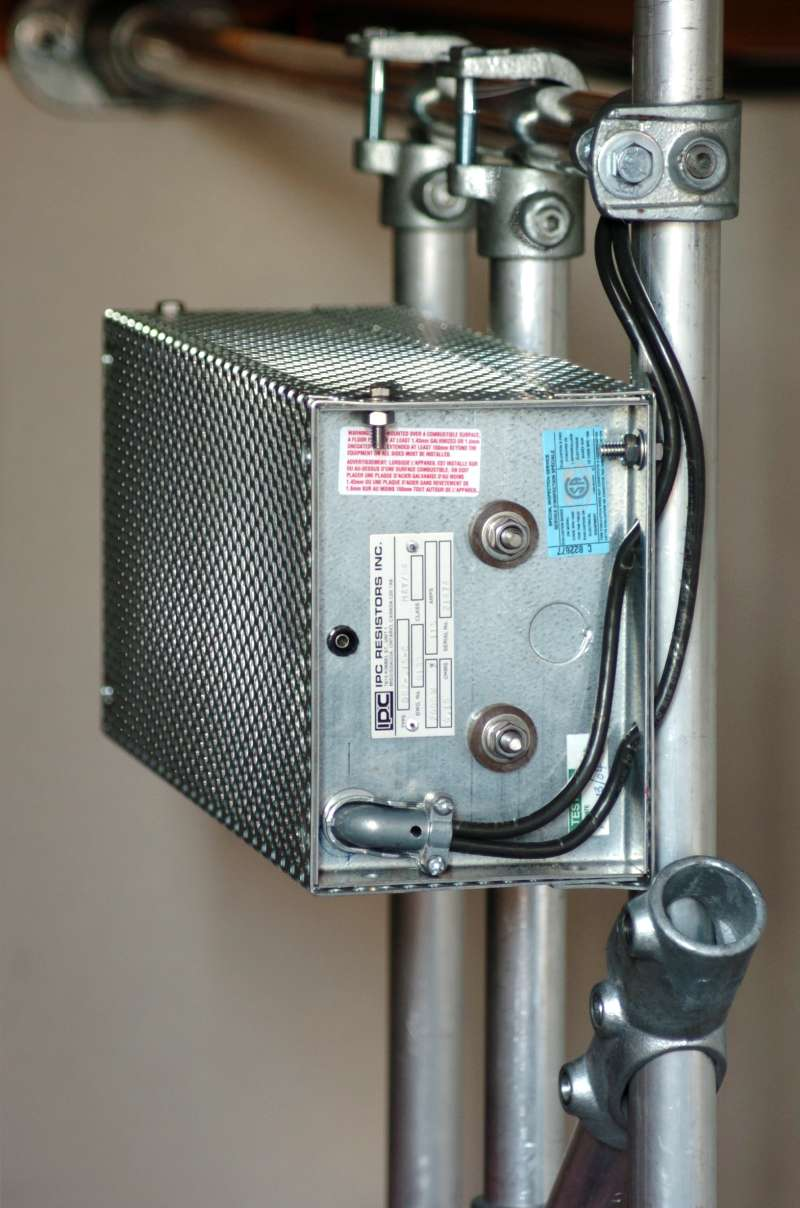
\includegraphics[height=1.3cm]{../../figures/d3_brake_resistor.jpg}}\\
\credit{brake resistor: Glogger, CC BY-SA 3.0, via Wikimedia Commons}
\end{column}
\end{columns}
\end{frame}

% --------------------------------------------------------------------
\begin{frame}{Power switches and dead time}
\begin{columns}[T]
\begin{column}{.62\textwidth}
\small
\begin{tabularx}{\linewidth}{@{}l X X X@{}}
\toprule
 & \textbf{Si IGBT} & \textbf{Si MOSFET} & \textbf{SiC MOSFET}\\
\midrule
voltage & 600--1700\,V & $\le$ 250\,V & 650--1700\,V\\
switching & slower & very fast & very fast\\
typ.\ $f_{sw}$ & 4--16\,kHz & 20--100\,kHz & 16--100\,kHz\\
used in & 400\,V drives & 24--72\,V cobots, AMRs & compact drives\\
\bottomrule
\end{tabularx}
\vspace{2mm}
\begin{itemize}\setlength\itemsep{.3mm}
\item \term{dead time} $t_d$ (0.5--3\,\si{\micro s}): both switches of a leg off at every change, to avoid \term{shoot-through} (a short circuit of the DC bus)
\item price: a small voltage error $\Delta\bar v\approx t_d\,f_{sw}\,V_{dc}$
\item example: $1\,\si{\micro s}\cdot16\,\text{kHz}\cdot325\,\text{V}=\SI{5.2}{V}$
\end{itemize}
\end{column}
\begin{column}{.36\textwidth}
\centering
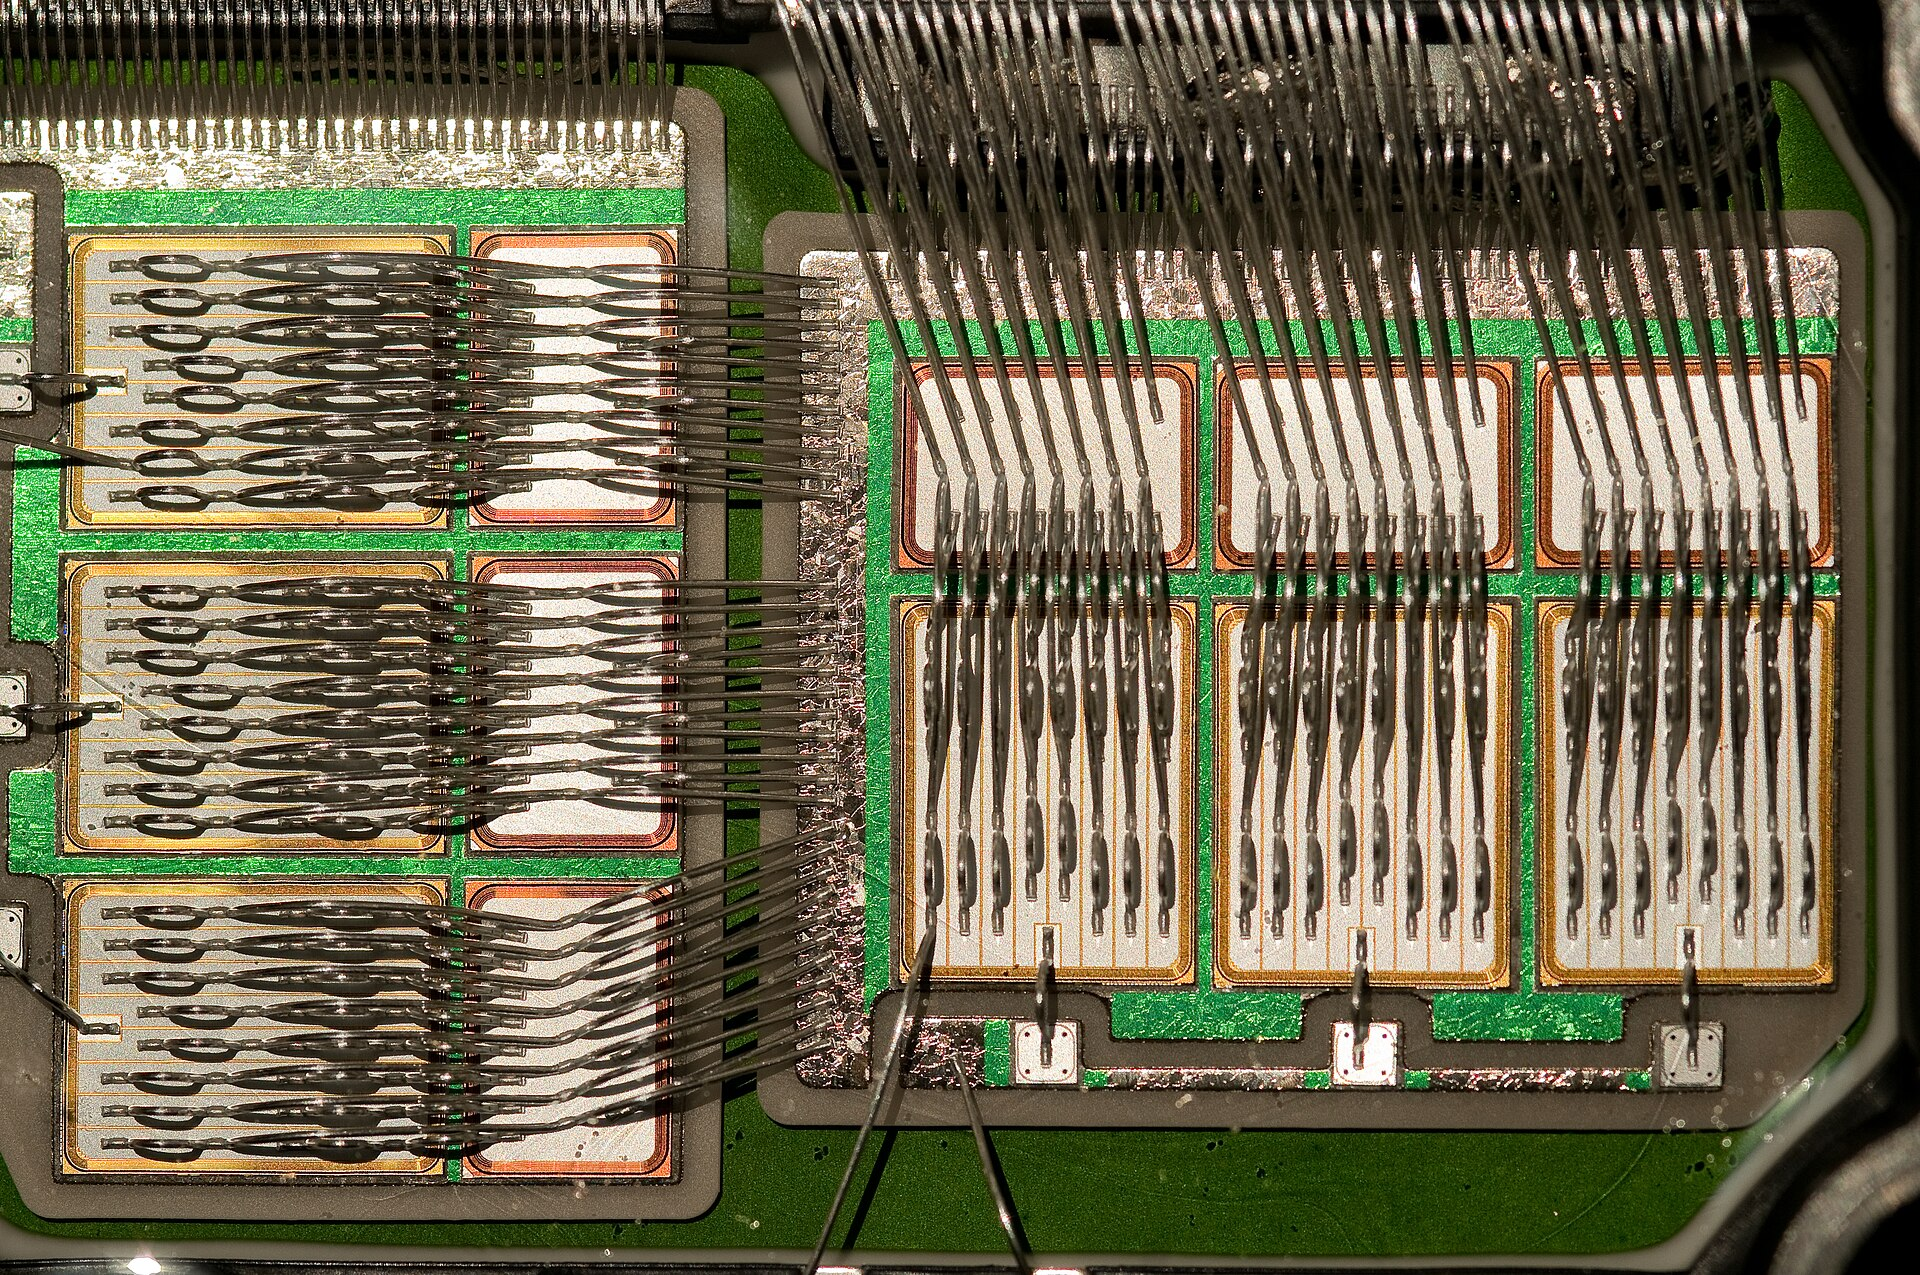
\includegraphics[width=\linewidth]{../../figures/d3_igbt_module_open.jpg}\\
\credit{Pslawinski, CC BY-SA 3.0, via Wikimedia Commons}\\
{\scriptsize opened IGBT module: chips and bond wires}
\end{column}
\end{columns}
\src{[Mohan, Undeland \& Robbins, 2003, ch.~8]; [Krishnan, 2001].}
\end{frame}

% --------------------------------------------------------------------
\begin{frame}{Session 3.2 --- Check your understanding}
\begin{keybox}[Check your understanding]
\begin{enumerate}\setlength\itemsep{2mm}
\item Why can a servo drive not simply use a ``half-on'' transistor, like a variable resistor, to set the motor voltage?
\item A 48\,V joint drive needs an average of 12\,V. What duty cycle does it use?
\item A drive trips on DC-bus over-voltage only while the robot lowers a heavy part. What is missing or too small?
\end{enumerate}
\end{keybox}
\vspace{2mm}
{\small\color{mkGray}Discuss in pairs for 2 minutes, then we compare answers.}
\end{frame}

% --------------------------------------------------------------------
\begin{frame}{Session 3.2 --- Summary and key terms}
\begin{columns}[T]
\begin{column}{.52\textwidth}
\begin{keybox}[Key take-aways]
\begin{itemize}\setlength\itemsep{.3mm}
\item Rectifier $\rightarrow$ DC bus $\rightarrow$ brake chopper $\rightarrow$ inverter $\rightarrow$ motor.
\item $V_{dc}\approx1.35\,V_{LL}$: 540\,V at 400\,V mains.
\item PWM: $\bar v=D\,V_{dc}$; the inverter makes sines from it.
\item Current limit sets torque; voltage limit sets top speed.
\item Braking energy goes into $R_b$, not the capacitor.
\end{itemize}
\end{keybox}
\end{column}
\begin{column}{.46\textwidth}
\begin{defbox}[Key terms]
\small
\term{DC bus} capacitor-backed DC link $\cdot$ \term{inverter} DC to 3-phase AC $\cdot$ \term{PWM} on/off switching with variable on-time $\cdot$ \term{duty cycle} on-time fraction $\cdot$ \term{regeneration} motor feeding energy back $\cdot$ \term{brake chopper} switch + resistor that burns it $\cdot$ \term{shoot-through} both switches of a leg on
\end{defbox}
\end{column}
\end{columns}
\end{frame}

% ====================================================================  closing
\section*{Wrap-up}
\begin{frame}{Day summary}
\begin{columns}[T]
\begin{column}{.5\textwidth}
\begin{defbox}[Control (2.7--2.9)]
\small
\begin{itemize}\setlength\itemsep{.3mm}
\item filters cost phase; notches remove resonances; lead buys phase back
\item sampling delay $\approx1.5T$ costs $360^\circ f_cT_d$
\item robot arms: independent joints + gravity compensation; computed torque and impedance control for demanding tasks
\end{itemize}
\end{defbox}
\end{column}
\begin{column}{.48\textwidth}
\begin{defbox}[Servo hardware (3.1--3.2)]
\small
\begin{itemize}\setlength\itemsep{.3mm}
\item drive + motor + gearbox + encoder + controller, one per joint
\item torque / velocity / position modes; cascaded loops
\item rectifier, DC bus, PWM inverter, brake chopper
\end{itemize}
\end{defbox}
\begin{keybox}[One sentence]
A robot joint is a servo axis whose bandwidth is limited by phase: filters, delay and resonances spend it; compensators and fast sampling buy it back.
\end{keybox}
\end{column}
\end{columns}
\end{frame}

\begin{frame}{Preview of W1D5: Servo Systems II}
\begin{columns}[T]
\begin{column}{.55\textwidth}
\small
\begin{itemize}\setlength\itemsep{.5mm}
\item 3.3 Field-oriented control: Clarke/Park, $i_d$ and $i_q$ currents
\item 3.4 Cascaded current, velocity and position loops in detail
\item 3.5 Loop tuning and bandwidth: inner $\rightarrow$ outer, inertia ratio, delays
\item 3.6 Trajectory generation, feedforward and disturbance compensation
\end{itemize}
\end{column}
\begin{column}{.43\textwidth}
\begin{notebox}
\small \textbf{Bring with you:} the delay formula $360^\circ f_cT_d$, the cascade structure, the inverter and $\bar v=D\,V_{dc}$ --- tomorrow we tune exactly these loops.
\end{notebox}
\end{column}
\end{columns}
\end{frame}

\begin{frame}{Figure credits}
\scriptsize
All other diagrams and plots: own drawings, computed for this course (TikZ / pgfplots / circuitikz).\\[1mm]
\begin{tabularx}{\textwidth}{@{}l X l@{}}
\toprule
\textbf{File} & \textbf{Source (Wikimedia Commons)} & \textbf{Author, licence}\\
\midrule
d3\_aliasing.png & File:AliasingSines.svg & Moxfyre, CC BY-SA 3.0\\
d3\_servo\_drive\_motor.jpg & File:Yeskawa Servo Drive \& Motor.jpg & Projuktiponno, CC BY-SA 4.0\\
d3\_servo\_drives.png & File:Servo motor drive.png & Tero Kontkanen, CC BY-SA 3.0\\
d4\_kuka\_robot.jpg & File:KUKA industrial robotic arm performing ``The Beach'' by Roy Nachum - 02.jpg & Oleg Yunakov, CC BY-SA 4.0\\
d1\_harmonic\_drive.jpg & File:Harmonic Drive AG strain wave gear set.jpg & Pieceofmetalwork, CC BY-SA 4.0\\
d3\_brake\_resistor.jpg & File:Turbrake.jpg & Glogger at English Wikipedia, CC BY-SA 3.0\\
d3\_igbt\_module\_open.jpg & File:CM600DU-24NFH.jpg & Pslawinski, CC BY-SA 3.0\\
r14\_cobot.jpg & File:Cobot.jpg (cropped) & GrowSkills Robotics, CC BY-SA 4.0\\
\bottomrule
\end{tabularx}
\end{frame}

\begin{frame}{References}
\fontsize{7}{8.4}\selectfont
\begin{columns}[T]
\begin{column}{.5\textwidth}
\begin{itemize}\setlength\itemsep{.2mm}
\item K.~Ogata, \emph{Modern Control Engineering}, 5th ed., Prentice Hall, 2010.
\item G.~F.~Franklin, J.~D.~Powell, A.~Emami-Naeini, \emph{Feedback Control of Dynamic Systems}, 8th ed., Pearson, 2019.
\item G.~F.~Franklin, J.~D.~Powell, M.~Workman, \emph{Digital Control of Dynamic Systems}, 3rd ed., Addison-Wesley, 1998.
\item K.~J.~{\AA}str\"om, R.~M.~Murray, \emph{Feedback Systems}, 2nd ed., Princeton Univ.\ Press, 2021.
\item K.~J.~{\AA}str\"om, T.~H\"agglund, \emph{Advanced PID Control}, ISA, 2006.
\item G.~Ellis, \emph{Control System Design Guide}, 4th ed., Butterworth-Heinemann, 2012.
\item A.~V.~Oppenheim, R.~W.~Schafer, \emph{Discrete-Time Signal Processing}, 3rd ed., Pearson, 2010.
\end{itemize}
\end{column}
\begin{column}{.5\textwidth}
\begin{itemize}\setlength\itemsep{.2mm}
\item M.~W.~Spong, S.~Hutchinson, M.~Vidyasagar, \emph{Robot Modeling and Control}, 2nd ed., Wiley, 2020.
\item B.~Siciliano, L.~Sciavicco, L.~Villani, G.~Oriolo, \emph{Robotics: Modelling, Planning and Control}, Springer, 2009.
\item J.~J.~Craig, \emph{Introduction to Robotics: Mechanics and Control}, 4th ed., Pearson, 2018.
\item N.~Hogan, ``Impedance control: an approach to manipulation,'' \emph{ASME J.\ Dyn.\ Sys., Meas., Control}, 107(1), 1985.
\item N.~Mohan, T.~M.~Undeland, W.~P.~Robbins, \emph{Power Electronics: Converters, Applications and Design}, 3rd ed., Wiley, 2003.
\item R.~Krishnan, \emph{Electric Motor Drives: Modeling, Analysis, and Control}, Prentice Hall, 2001.
\item IEC 61800-5-1 (adjustable speed drives: safety); IEC 61800-7 (drive profiles).
\end{itemize}
\end{column}
\end{columns}
\end{frame}

\end{document}
